%%%%%%%%%%%%%%%%%%%%%%%%%%%%%%%%%%%%%%%%%
% University/School Laboratory Report
% LaTeX Template
% Version 3.1 (25/3/14)
%
% This template has been downloaded from:
% http://www.LaTeXTemplates.com
%
% Original author:
% Linux and Unix Users Group at Virginia Tech Wiki 
% (https://vtluug.org/wiki/Example_LaTeX_chem_lab_report)
%
% License:
% CC BY-NC-SA 3.0 (http://creativecommons.org/licenses/by-nc-sa/3.0/)
%
%%%%%%%%%%%%%%%%%%%%%%%%%%%%%%%%%%%%%%%%%

%----------------------------------------------------------------------------------------
%	PACKAGES AND DOCUMENT CONFIGURATIONS
%----------------------------------------------------------------------------------------

\documentclass{article}

\usepackage[version=3]{mhchem} % Package for chemical equation typesetting
\usepackage{siunitx} % Provides the \SI{}{} and \si{} command for typesetting SI units
\usepackage{graphicx} % Required for the inclusion of images
\usepackage{natbib} % Required to change bibliography style to APA
\usepackage{amsmath} % Required for some math elements 
\usepackage{enumerate} % Required for the enumerate function
\usepackage[siunitx]{circuitikz} % Required for the drawing of circuit diagrams
\usepackage{caption}
\usepackage{graphicx}
\usepackage{subcaption}
\usepackage{xfrac}
\usepackage{float}
\usepackage{enumitem}
\usepackage{chemgreek}
\usepackage{epstopdf}
\usepackage{tikz}
\usetikzlibrary{arrows}
\usepackage{booktabs}
\usepackage{capt-of}
\usepackage{ mathrsfs }


\setlength\parindent{0pt} % Removes all indentation from paragraphs

\renewcommand{\labelenumi}{\alph{enumi}.} % Make numbering in the enumerate environment by letter rather than number (e.g. section 6)

%\usepackage{times} % Uncomment to use the Times New Roman font

\topmargin=-0.45in
\evensidemargin=0in
\oddsidemargin=0in
\textwidth=6.5in
\textheight=9.0in
\headsep=0.25in

%----------------------------------------------------------------------------------------
%	DOCUMENT INFORMATION
%----------------------------------------------------------------------------------------

\title{Control Systems \\ Laboratory Report \\ ENG476} % Title

\author{Shane \textsc{Reynolds}} % Author name

\date{October 1, 2016} % Date for the report

\begin{document}

\maketitle % Insert the title, author and date

\begin{center}
\begin{tabular}{l r}
Date Performed: & September 09, 2016 \\ % Date the experiment was performed
Instructor: & Professor Friso De Boer % Instructor/supervisor
\end{tabular}
\end{center}

% If you wish to include an abstract, uncomment the lines below
% \begin{abstract}
% Abstract text
% \end{abstract}

\tableofcontents
\newpage
%----------------------------------------------------------------------------------------
%	SECTION 1
%----------------------------------------------------------------------------------------

\section{Modelling of a DC Servo Motor}

%----------------------------------------------------------------------------------------
%	SUBSECTION 1
%----------------------------------------------------------------------------------------

\subsection{Objective}

To capture experimental data from a physical system and determine the transfer function governing its behaviour.
 
%----------------------------------------------------------------------------------------
%	SUBSECTION 2
%----------------------------------------------------------------------------------------

\subsection{Procedure and Results}

The open loop block diagram of the physical system being analysed can be seen in Figure 1. A range of frequencies from 1$\si{\radian\per\second}$ through to 200$\si{\radian\per\second}$ were selected as frequencies for sinusoidal inputs for the system. Experimental data for the output waveforms were recorded. Figure 2 shows the input and output waveforms for the different frequencies.

\vspace{0.5cm}

\tikzstyle{int}=[draw, fill=blue!20, minimum height=4em, text width=5em, text centered]
\tikzstyle{init} = [pin edge={to-,thin,black}]
\begin{figure}[H]
	\centering
	\begin{tikzpicture}[node distance=2.5cm,auto,>=latex']
	\node [int] (b) {D2A};
	\node (a) [left of=b,node distance=2cm, coordinate] {input};
	\node [int] (c) [right of=b] {Amplifier Gain $K$};
	\node [int] (d) [right of=c] {Motor \& Gears};
	\node [int] (e) [right of=d] {Position Potentiometer};
	\node [int] (f) [below of=d] {Tacho};
	\node [int] (g) [right of=f] {A2D};
	\node [coordinate] (end) [right of=g, node distance=2cm]{};
	
	\path[->] (a) edge node {$u(t)$} (b);
	\path[->] (b) edge node {} (c);
	\path[->] (c) edge node {} (d);
	\path[->] (d) edge node {} (e);
	\path[->] (d) edge node {} (f);
	\path[->] (f) edge node {} (g);
	\path[->] (e) edge node {} (g);
	\path[->] (g) edge node {$y(t)$} (end);
	\end{tikzpicture}
	\caption{Open loop block diagram for the experimental setup.}
\end{figure}

Two methods were used to determine the magnitude and phase of the system transfer function for the chosen frequencies. The first method employed linear regression to fit a sinusoidal curve to the data, which allowed for accurate estimation of the waveform amplitudes. The phase was found using a statistical technique. The second technique employed the use of the Fast Fourier Transform. The results for each method can be seen in Tables 1 \& 2.\\

A Bode plots of the determined magnitudes and phases from the first and second method can be seen in Figure 5 and 6, respectively. The statistical method that was used to obtain the phase in the first method appears to be somewhat unreliable for higher order frequencies, which manifests as erratic data points seen in the phase plot of Figure 3. This problem does not occur with the second method, using the Fast Fourier Transform - the plot of which can be seen in Figure 4.\\

The system was modelled using a second order transfer function of the following form:
\begin{align*}
H(s) = \frac{K}{s \cdot (\tau \cdot s + 1)}
\end{align*}

Using the data from the first method, the transfer function was fit using the system identification toolbox in MATLAB. The transfer function of best fit, with a reported accuracy of 88.56\%, was:
\begin{align}
H(s) = \frac{1.91}{s(0.025s + 1)}
\end{align}

Similarly, a transfer function was fit using the data from the second method. The transfer function of best fit, with a reported accuracy of 88.42\%, was:
\begin{align}
H(s) = \frac{1.94}{s(0.034s + 1)}
\end{align}

\begin{figure}[H]
	\hspace{-3.5cm}
	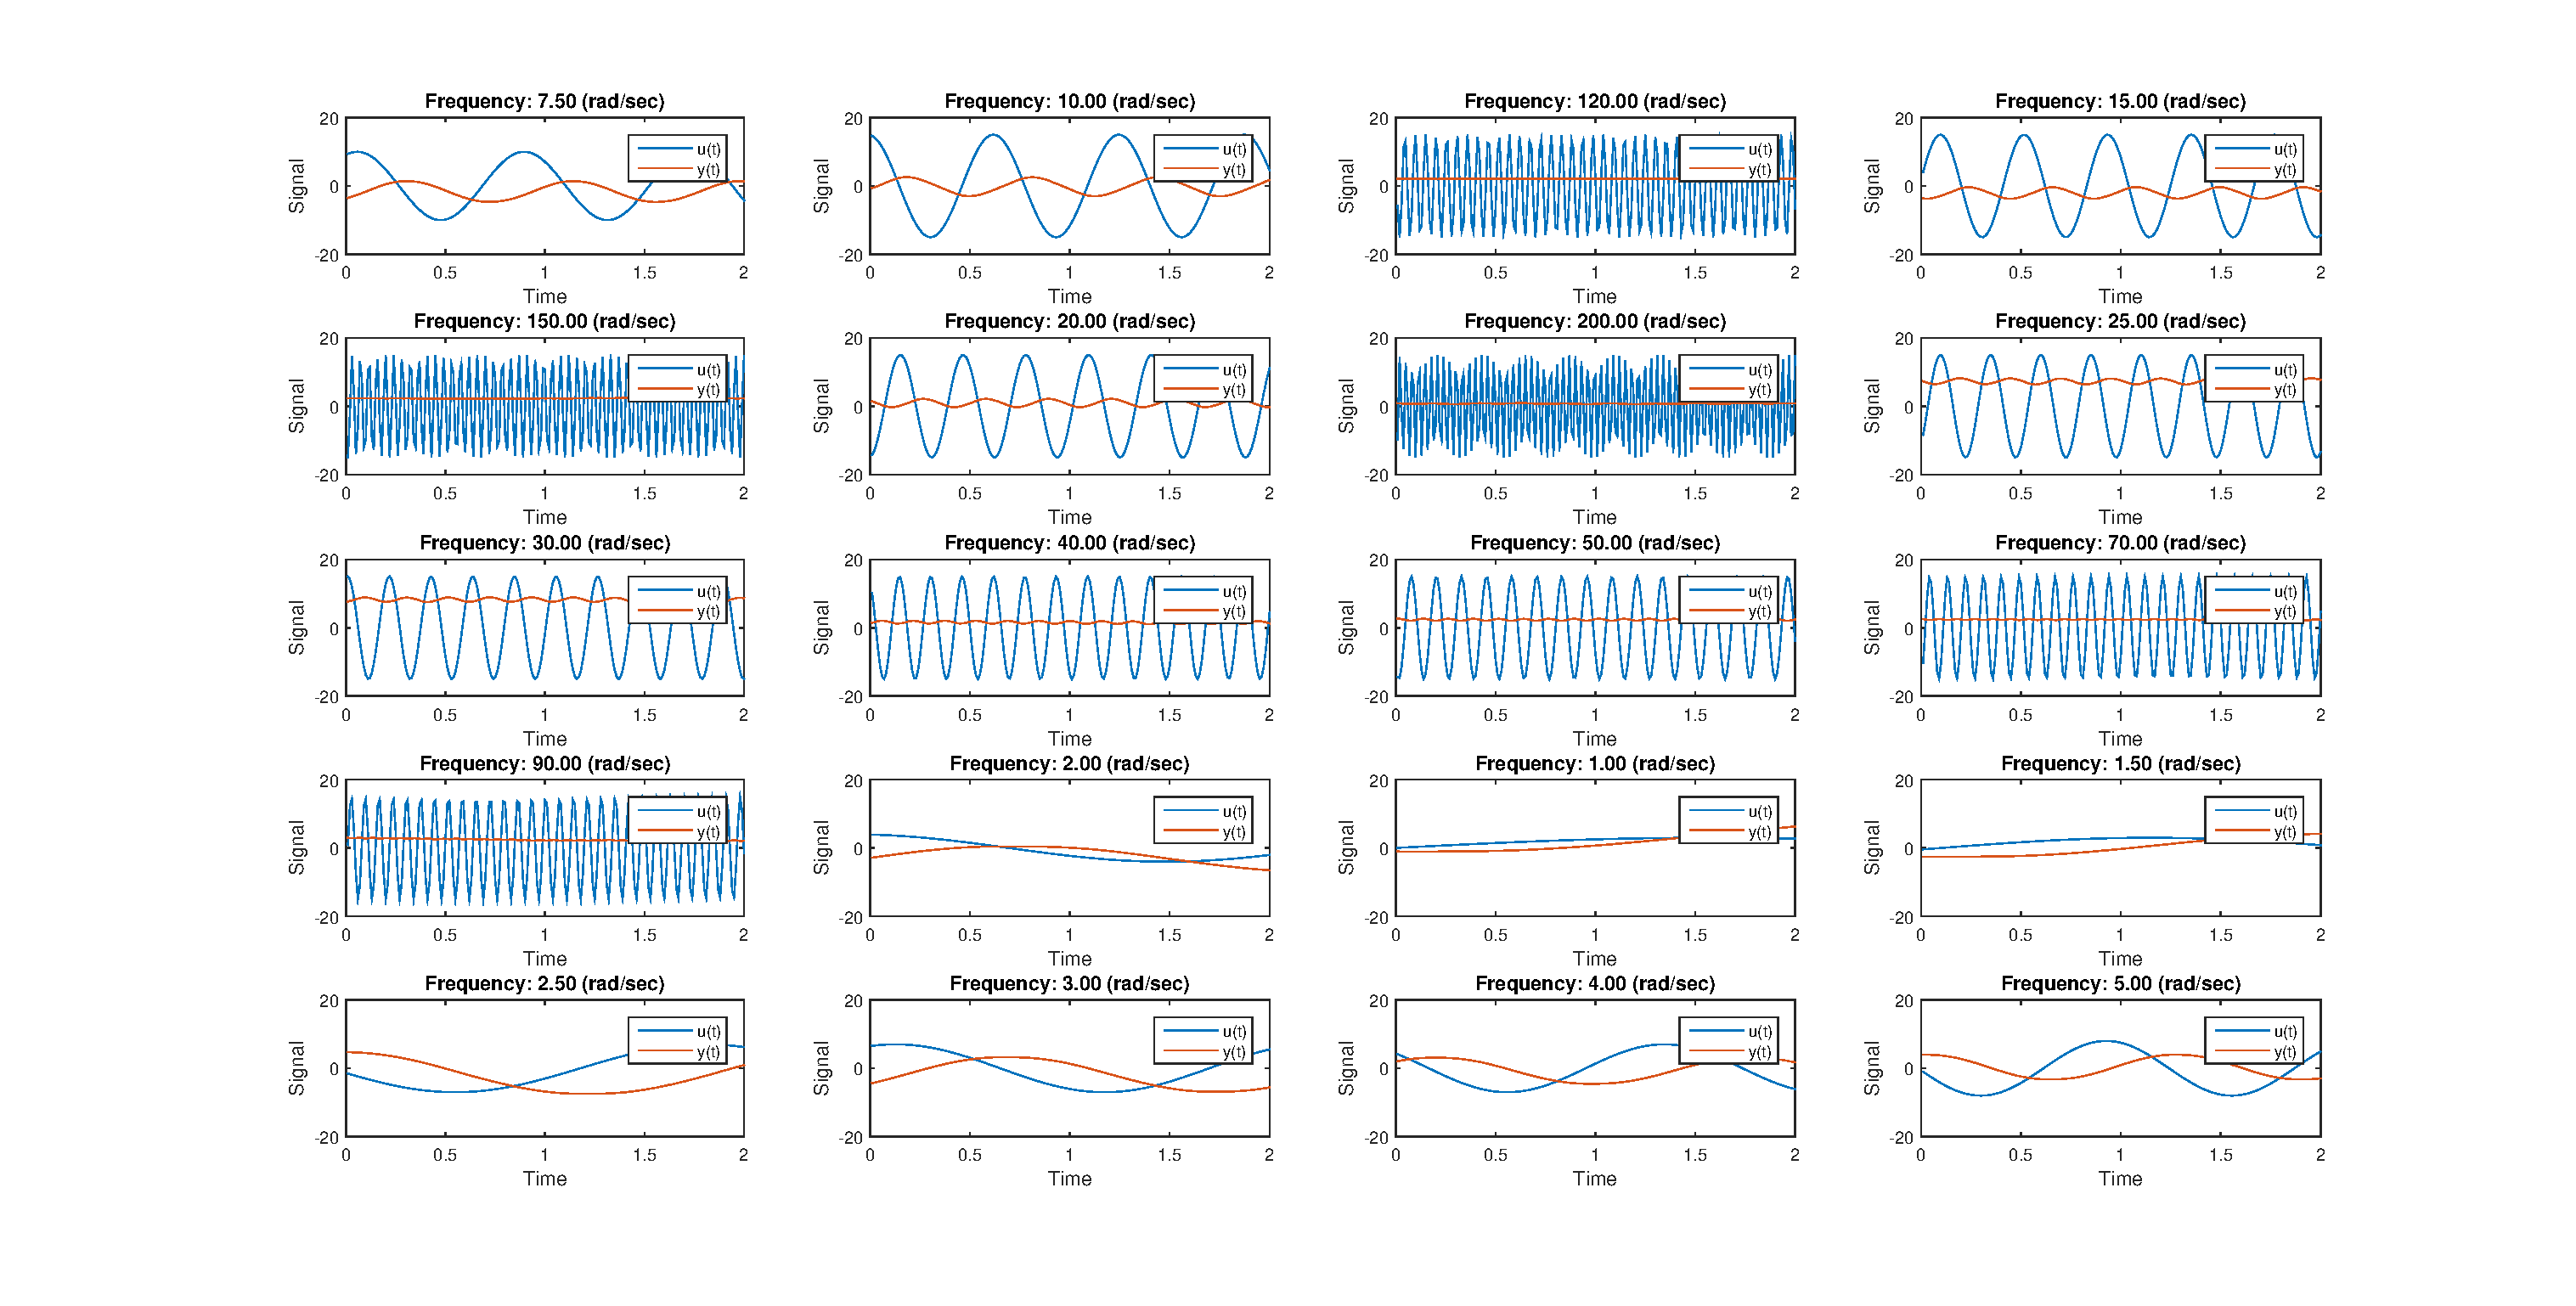
\includegraphics[scale=0.45]{fig1}
	\caption{Plots showing the input and output sinusoidal waveforms.}
\end{figure}

\begin{figure}[H]
	\hspace{0.5cm}
	\begin{minipage}{7cm}
		\centering
		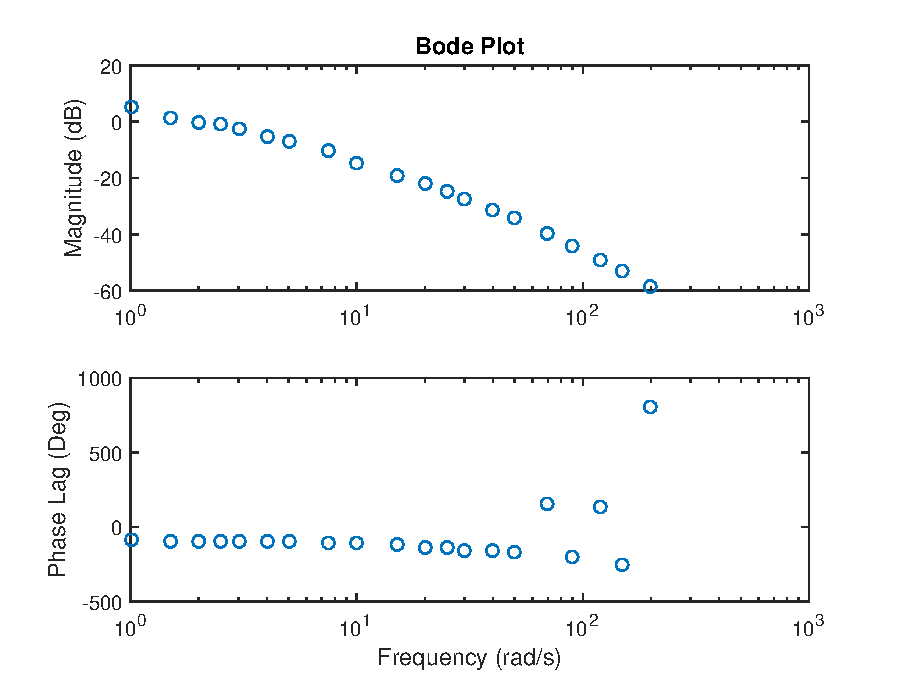
\includegraphics[scale=0.5]{fig3}
		\caption{Bode diagram of experimental data from transfer function amplitudes and phases found using method 1.}
	\end{minipage}
	\hspace{1cm}
	\begin{minipage}{7cm}
		\centering
		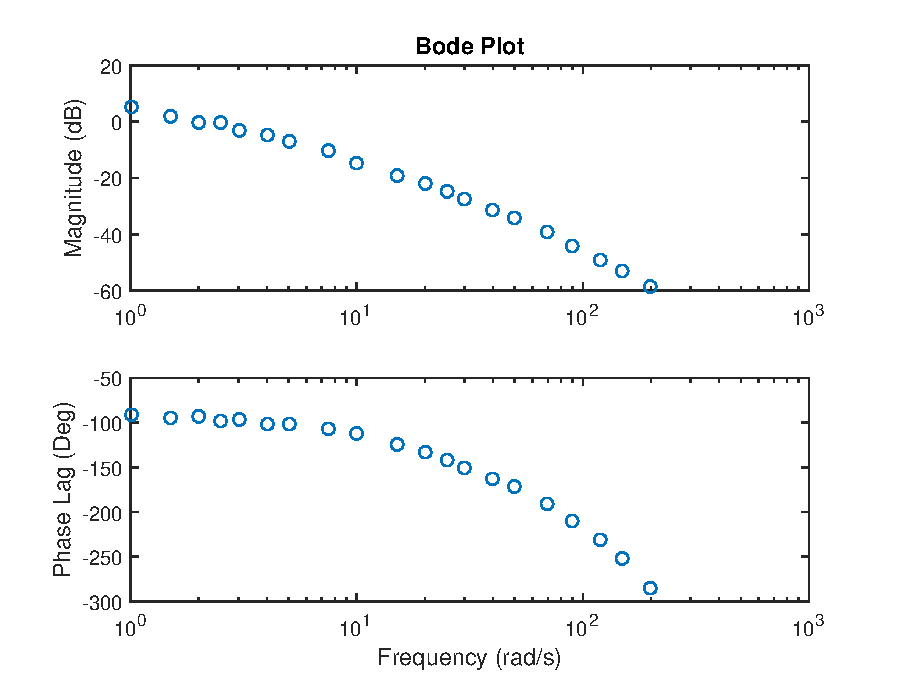
\includegraphics[scale=0.5]{fig5}
		\caption{Bode diagram of experimental data from transfer function amplitudes and phases found using method 2.}
	\end{minipage}	
\end{figure}

\begin{table}[H]
	\hspace{0.5cm}
	\begin{minipage}{7cm}
		\centering
		\caption{Transfer function magnitude\\ for both methods of estimation.}
		\begin{tabular}{rrr}
			\toprule
			\multicolumn{1}{c}{\textbf{Frequency}} & 
			\multicolumn{1}{c}{\textbf{Method 1}} & \multicolumn{1}{c}{\textbf{Method 2}}\\
			\multicolumn{1}{c}{($\mathbf{\si{\radian\per\second}}$)} & 
			\multicolumn{1}{c}{$|H(\omega)|$} & \multicolumn{1}{c}{$|H(\omega)|$}\\
			\midrule
			1.00    &	1.8218	&	1.8344\\
			1.50    &	1.2023	&	1.2541\\
			2.00    &	0.9653	&	0.9728\\
			2.50    &	0.8960	&	0.9389\\
			3.00    &	0.7425	&	0.7251\\
			4.00    &	0.5607	&	0.5710\\
			5.00    &	0.4623	&	0.4615\\
			7.50    &	0.3053	&	0.3043\\
			10.00   &	0.1793	&	0.1793\\
			15.00   & 	0.1097	&	0.1083\\
			20.00   & 	0.0793	&	0.0791\\
			25.00   & 	0.0569	&	0.0572\\
			30.00   & 	0.0430	&	0.0428\\
			40.00   & 	0.0276	&	0.0276\\
			50.00   & 	0.0193	&	0.0193\\
			70.00   & 	0.0104	&	0.0107\\
			90.00   & 	0.0061	&	0.0061\\
			120.00  &  	0.0035	&	0.0034\\
			150.00  &  	0.0022	&	0.0023\\
			200.00  &  	0.0012	&	0.0011\\
			\bottomrule
		\end{tabular}
	\end{minipage}
	\hspace{1cm}
	\begin{minipage}{7cm}
		\centering
		\caption{Transfer function phase\\ for both methods of estimation.}
		\begin{tabular}{rrr}
			\toprule
			\multicolumn{1}{c}{\textbf{Frequency}} & 
			\multicolumn{1}{c}{\textbf{Method 1}} & \multicolumn{1}{c}{\textbf{Method 2}}\\
			\multicolumn{1}{c}{($\mathbf{\si{\radian\per\second}}$)} & 
			\multicolumn{1}{c}{$\angle\big(H(\omega)\big)$} & \multicolumn{1}{c}{$\angle\big(H(\omega)\big)$}\\
			\midrule
			1.00	&	-90.52		&	-91.78\\
			1.50	&	-92.81		&	-94.68\\
			2.00	&	-91.67		&	-92.67\\
			2.50	&	-94.53		&	-97.28\\
			3.00	&	-94.53		&	-95.90\\
			4.00	&	-98.54		&	-101.88\\
			5.00	&	-100.26		&	-101.49\\
			7.50	&	-107.42		&	-106.52\\
			10.00	&	-108.86		&	-111.99\\
			15.00	&	-120.32		&	-124.15\\
			20.00	&	-137.50		&	-132.50\\
			25.00	&	-143.23		&	-142.64\\
			30.00	&	-154.69		&	-150.25\\
			40.00	&	-160.42		&	-162.77\\
			50.00	&	-171.88		&	-172.29\\
			70.00	&	160.42		&	-191.43\\
			90.00	&	-206.26		&	-209.46\\
			120.00	&	137.50		&	-230.44\\
			150.00	&	-257.83		&	-251.87\\
			200.00	&	802.14		&	-284.63\\
			\bottomrule
		\end{tabular}
	\end{minipage}
\end{table}

\begin{figure}[H]
	\hspace{0.5cm}
	\begin{minipage}{7cm}
		\centering
		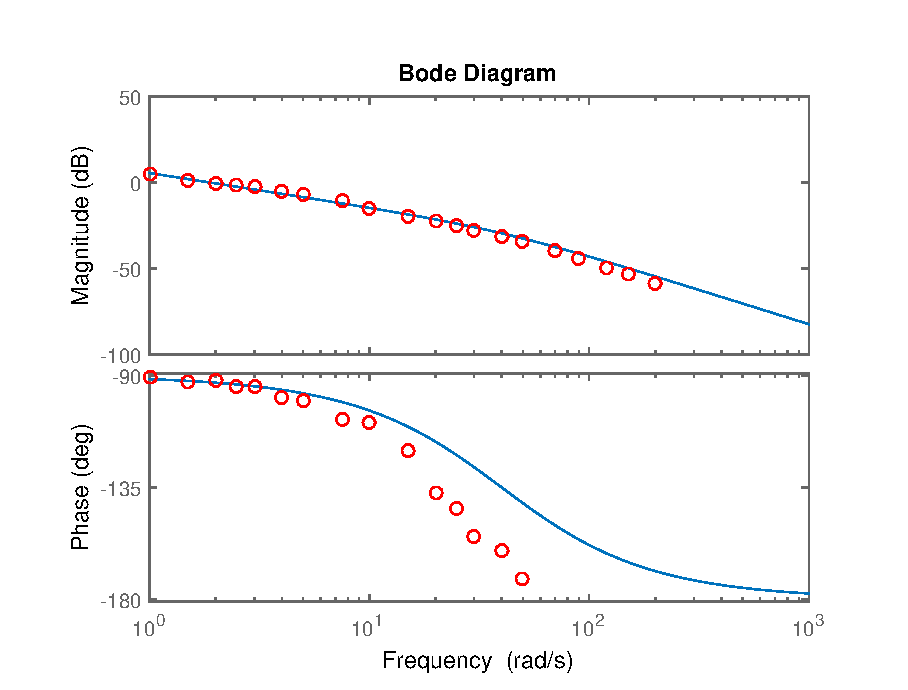
\includegraphics[scale=0.5]{fig2}
		\caption{Bode diagram of transfer function and experimental data from transfer function amplitudes and phases found using method 1.}
	\end{minipage}
	\hspace{1cm}
	\begin{minipage}{7cm}
		\centering
		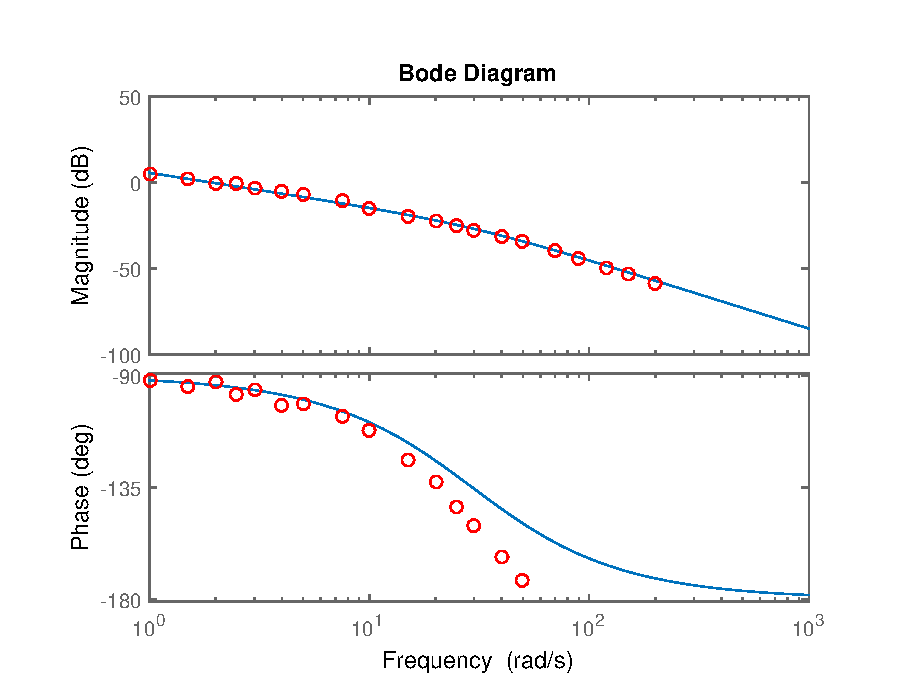
\includegraphics[scale=0.5]{fig4}
		\caption{Bode diagram of transfer function and experimental data from transfer function amplitudes and phases found using method 2.}
	\end{minipage}	
\end{figure} 
\newpage
%----------------------------------------------------------------------------------------
%	SECTION 2
%----------------------------------------------------------------------------------------

\section{Proportional Feedback Control}

%----------------------------------------------------------------------------------------
%	SUBSECTION 1
%----------------------------------------------------------------------------------------

\subsection{Objective}

To analyse the performance of a physical system which is being controlled using proportional position feedback control.

%----------------------------------------------------------------------------------------
%	SUBSECTION 2
%----------------------------------------------------------------------------------------

\subsection{Procedure and Results}

The transfer function for the open loop system determined in section 1 is used to represent the plant, $G_P$, of the system being controlled. The block diagram detailing the topology for proportional position feedback control, $G_C$, can be seen in Figure 7.

\tikzstyle{int}=[draw, fill=blue!20, minimum height=4em, text width=5em, text centered]
\tikzstyle{sum} = [draw, fill=white, circle, node distance=1cm]
\tikzstyle{init} = [pin edge={to-,thin,black}]
\begin{figure}[H]
	\centering
	\begin{tikzpicture}[node distance=3.5cm,auto,>=latex']
	\node [sum] (b) {};
	\node (a) [left of=b,node distance=1.5cm, coordinate] {input};
	\node [int] (c) [right of=b,node distance=2.5cm] {$G_C = K_P$};
	\node [int] (d) [right of=c] {$G_P$};
	\node [coordinate] (end) [right of=d, node distance=3.5cm]{};
	
	
	\path[->] (a) edge node {$r(t)$} (b);
	\path[->] (b) edge node {$e(t)$} (c);
	%\path[->] (c) edge node {} (d);
	\draw [->] (c) -- node [name=u] {$u(t)$}(d);
	
	\node [int] (unit) [below of=u] {1};
	
	%\path[->] (d) edge node {$y(t)$} (end);
	\draw [->] (d) -- node [name=y] {$y(t)$}(end);
	\draw [->] (y) |- (unit);
	\draw [->] (unit) -| node[pos=0.99] {$-$} node [near end] {$y(t)$} (b);
	\end{tikzpicture}
	\caption{Open loop block diagram for the experimental setup.}
\end{figure}

Velocity feedback was set to zero and a step input to the system bewteen 0 and 1 was selected as input. The position feedback gain, $K_P$, was tuned such that a 16\% overshoot was obtained. The gain of the position feedback at this level was recorded as:
\begin{align*}
	K_P = 11.5
\end{align*}

A plot of the step response with $K_P = 11.5$ can be seen in Figure 8. The system was also fitted with an eddy current braking system. Step response data was recorded for the system operating with the brake engaged. Figure 9 shows the plot of the step response. Using the plots in Figures 8 and 9 estimates for the delay time ($t_d$), rise time ($t_r$), overshoot ($M_P$), and settling time ($t_s$) were found. The results can be seen in Table 3.
\vspace{0.5cm}
\begin{table}[H]
	\centering
	\caption{Performance metrics of position feedback controller.}
	\begin{tabular}{crr}
		\toprule
		\textbf{Parameter} & \textbf{Brake disengaged} & \textbf{Brake engaged}\\
		\midrule
		$t_d$ ($\si{\second}$) & 0.065 & 0.070\\
		$t_r$ ($\si{\second}$) & 0.100 & 0.160\\
		$M_P$ (\%) & 16 & 0\\
		$t_s$ ($\si{\second}$) & 0.230 & 0.160\\
		\bottomrule
	\end{tabular}
\end{table}

\begin{figure}[H]
	\hspace{0.5cm}
	\begin{minipage}{7cm}
		\centering
		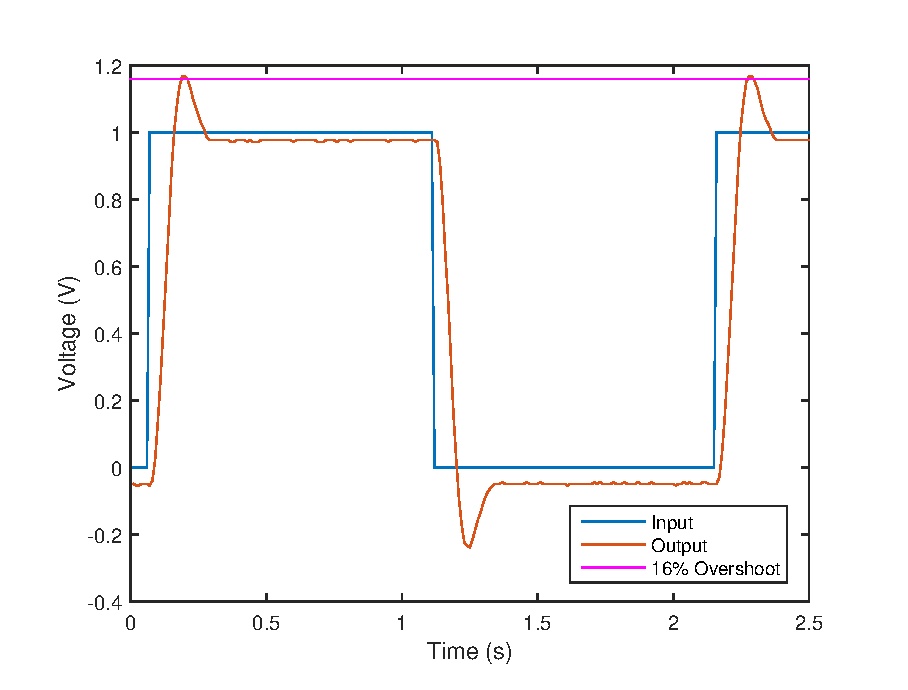
\includegraphics[scale=0.5]{fig6}
		\caption{Step response of system with positional feedback $K_P = 11.5$, providing a maximum overshoot of 16\%.}
	\end{minipage}
	\hspace{1cm}
	\begin{minipage}{7cm}
		\centering
		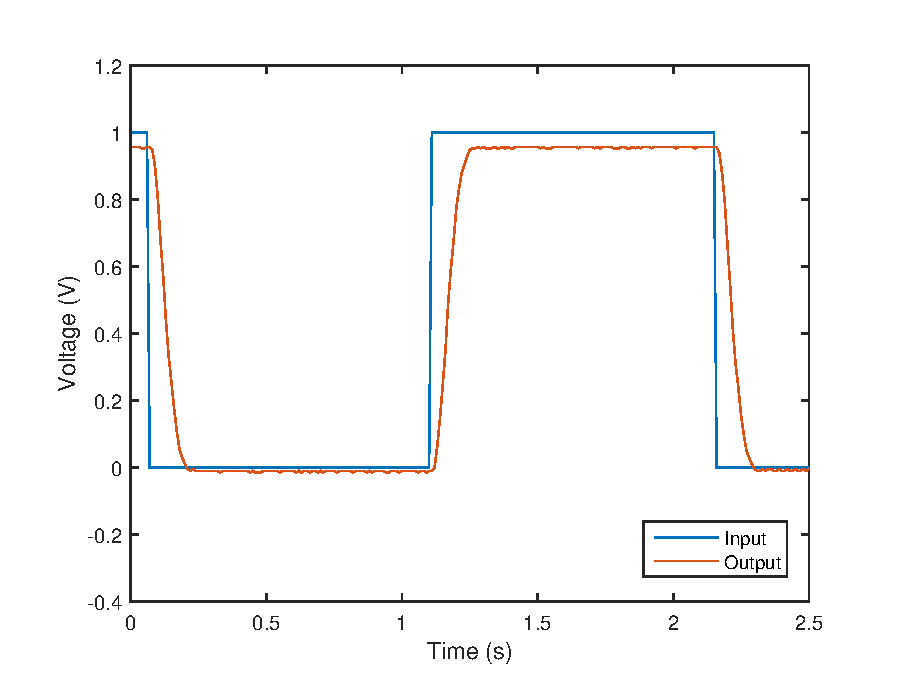
\includegraphics[scale=0.5]{fig7}
		\caption{Step response of system with positional feedback $K_P = 11.5$, with the eddy current brake engaged.}
	\end{minipage}
\end{figure}

The plots in Figure 8 and 9 show that the eddy current brake provides a dampening effect on the system. This is further emphasised through the metrics estimated from the plots in Table 3. Specifically there is no overshoot with the eddy current brake engaged, and the system tends to perform more sluggishly, with delay and rise times slower than the system without the brake engaged. Data was collected with the brake disengaged in order to find a transfer function describing the system with positional feedback control. A second order model was fit to the system, using the standard form:
\begin{align}
	H(s) = \frac{\omega_n^2}{s^2 + 2 \zeta \omega_n + \omega_n^2}
\end{align}

The Fast Fourier technique from Section 1 was used in addition with the system identification toolbox. The transfer function was fit according to equation (3) with a reported 83.09\% accuracy. Further manual adjustment of the parameters, combined with visual inspection yielded the following transfer function:
\begin{align}
H(s) = \frac{595}{s^2 + 20.75s + 595}
\end{align}

A step response was simulated using the empirically determined transfer function shown in equation (4). A plot of the results can be seen in Figure 10, which provides for comparison between the simulation and the actual step response of the system. In the plot we can see that the empirical data of a single step follows the experimentally determined transfer function quite closely, however, this is no surprise as the function itself was fit to the frequency response of this experimental data.\\

The root locus diagram for the open loop transfer function shown in equation (1) can be seen in Figure 11. Given that the overshoot, $M_P$, is 16 \%, the poles can be found by first estimating $\zeta$, and then finding $\omega_n$, using the coefficient $2 \cdot \zeta \cdot \omega_n$ from the denominator of a theoretically derived closed loop transfer function for the controlled system. Firstly, Ogata (2010) suggests that the overshoot can be found from equation (5):
\begin{align}
M_P &= e^{-\frac{\zeta}{\sqrt{1-\zeta^2}}}
\end{align}

\begin{figure}[H]
	\hspace{0.5cm}
	\begin{minipage}{7cm}
		\centering
		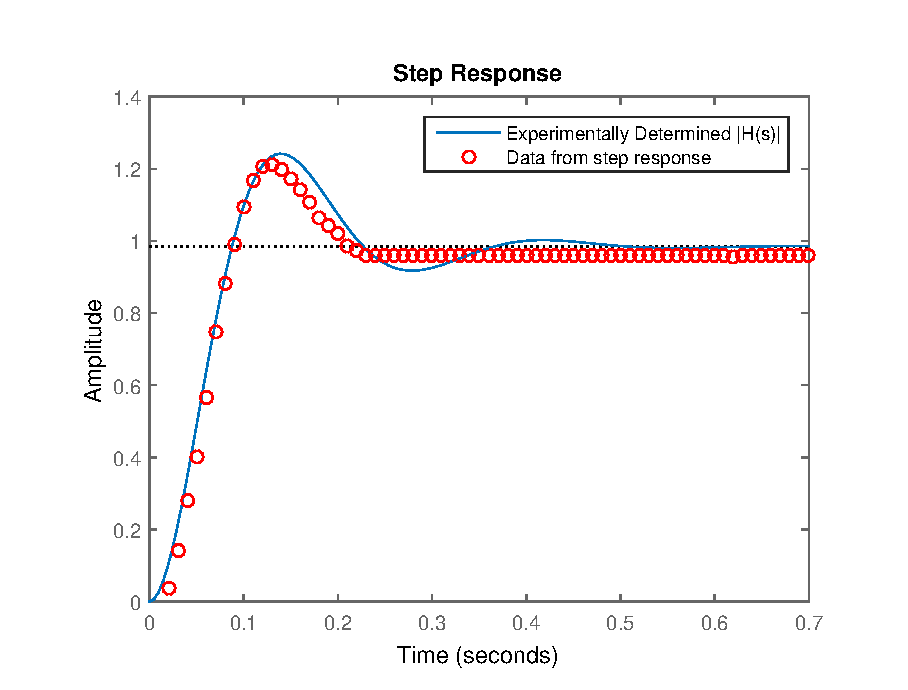
\includegraphics[scale=0.5]{fig8}
		\caption{Step response of the experimentally determined second order transfer function for the closed loop position feedback control system, shown in equation (4).}
	\end{minipage}
	\hspace{1cm}
	\begin{minipage}{7cm}
		\centering
		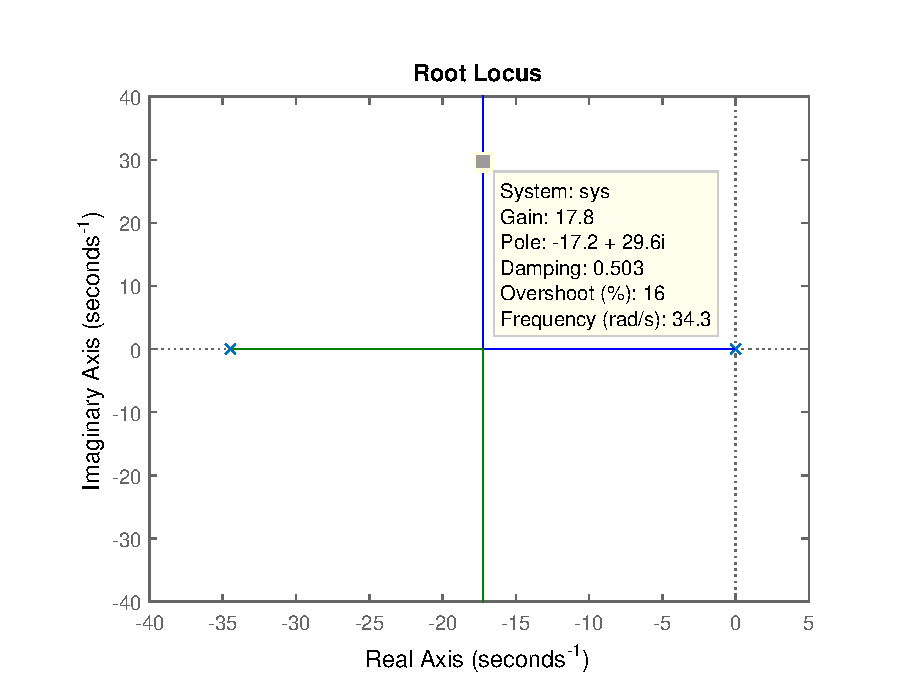
\includegraphics[scale=0.5]{fig9}
		\caption{Root locus diagram of the open loop transfer function shown by equation (1). The gain at the poles determined for a 16\% overshoot is 17.8.}
	\end{minipage}
\end{figure}



Rearranging equation (5), we get:
\begin{align*}
	\zeta  	&= \sqrt{\frac{\big(\frac{1}{\pi} \cdot \ln(M_P)\big)^2}{1 + \big(\frac{1}{\pi} \cdot \ln(M_P)\big)^2}}\\
			&= 0.5038
\end{align*}

Now, the closed loop transfer function is of the form:
\begin{align*}
	H(s) = \frac{K_P \cdot G(s)_P}{1 + K_P \cdot G(s)_P}
\end{align*}

Using the open loop transfer function from equation (1), we get the closed loop transfer function:
\begin{align}
	H(s) = \frac{K_P \cdot 65.86}{s^2 + 34.48s + K_P \cdot 65.86}
\end{align}

Hence, it can be seen that $2 \cdot \zeta \cdot \omega_n = 34.48$, and since $\zeta = 0.5038$, we get that:
\begin{align*}
	\omega_n = \frac{34.48}{2 \cdot 0.5038} = 34.21
\end{align*}

Solving the polynomial $s^2 + 2 (0.5038) (34.21)s + (34.21)^2 = 0$, we get the following two poles:
\begin{align*}
	p_1 &= -17.24 - i29.54\\
	p_2 &= -17.24 + i29.54
\end{align*}

The theoretical transfer function for the controlled system is given by:
\begin{align}
	H(f) = \frac{1191.63}{s^2 + 34.47s + 1170.32}
\end{align}

The gain at which these poles are located on the root locus diagram, shown in Figure 11, are at $K_P = 17.8$. This is approximately 50\% more gain than the experimentally determined gain of $K_P = 11.5$. The difference in the experimental gain and theoretical gain is dramatic, and may be due to a misspecified model or errors in the calculations. A bode plot shown in Figure 12 compares the experimentally determined transfer function in equation (4), and the theoretically determined one in equation (7). The differences between the theoretical model and the experimental model can be attributed to the difference in the gain previously reported. It must be noted that the experimental data follows the experimentally determined curve - perhaps if error in calculation is present then it is in the theoretical calculations.

\begin{figure}[H]
	\centering
	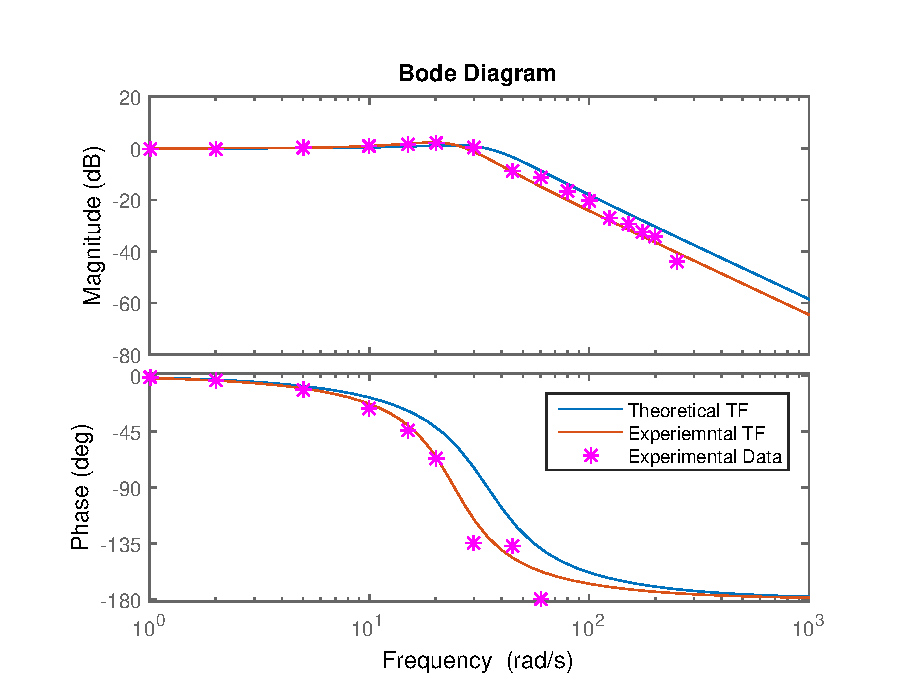
\includegraphics[scale=0.7]{fig10}
	\caption{text}
\end{figure}


%----------------------------------------------------------------------------------------
%	SECTION 3
%----------------------------------------------------------------------------------------

\section{Position and Velocity Feedback Control}

%----------------------------------------------------------------------------------------
%	SUBSECTION 1
%----------------------------------------------------------------------------------------

\subsection{Objective}

To analyse the influence of velocity feedback on a physical system which is being controlled using proportional position feedback control.

%----------------------------------------------------------------------------------------
%	SUBSECTION 2
%----------------------------------------------------------------------------------------

\subsection{Procedure and Results}

The transfer function for the open loop system determined in section 1 is used to represent the plant, $G_P$, of the system being controlled. The block diagram detailing the topology for velocity and proportional position feedback control can be seen in Figure 13.

\tikzstyle{int}=[draw, fill=blue!20, minimum height=4em, text width=5em, text centered]
\tikzstyle{sum} = [draw, fill=white, circle, node distance=1cm]
\tikzstyle{init} = [pin edge={to-,thin,black}]
\begin{figure}[H]\hspace{-0.5cm}
	\begin{tikzpicture}[node distance=3.5cm,auto,>=latex']
	\node [sum] (b) {};
	\node (a) [left of=b,node distance=1.5cm, coordinate] {input};
	\node [int] (c) [right of=b,node distance=2.5cm] {$K_P$};
	\node [sum] (d) [right of=c,node distance=2.5cm] {};
	\node [int] (e) [right of=d] {$G_P$};
	\node [int] (f) [right of=e] {$\frac{1}{s}$};
	\node [coordinate] (end) [right of=f, node distance=3.5cm]{};
	
	
	\path[->] (a) edge node {$r(t)$} (b);
	\path[->] (b) edge node {$e(t)$} (c);
	\path[->] (c) edge node {} (d);
	
	\path[->] (d) edge node {$u(t)$} (e);
	\draw [->] (e) -- node [name=n] {$\frac{d}{dt}y(t)$}(f);
	\draw [->] (f) -- node [name=m] {$y(t)$}(end);
	
	\node [int] (tacho) [below of=e, minimum height=3em, text width=3em, node distance=2.0cm] {$K_T$};
	\node [int] (velo) [left of=tacho, minimum height=3em, text width=3em, node distance=2.0cm] {$K_v$};
	\node [int] (unit) [below of=velo, node distance=2.0cm] {1};
	
	\draw [->] (m) |- (unit);
	\draw [->] (unit) -| node[pos=0.99] {$-$} node [near end] {$y(t)$} (b);
	\draw [->] (n) |- (tacho);
	\path [->] (tacho) edge node {} (velo);
	\draw [->] (velo) -| node[pos=0.99] {$-$} node [near end] {} (d);
	\end{tikzpicture}
	\caption{Open loop block diagram for the experimental setup.}
\end{figure}

In closed loop mode the controlled system was subjected to a step input between 0$\si{\volt}$ and 1$\si{\volt}$. The velocity feedback, $K_v$ was, set to 2 and $K_P$ was tuned to yield 16\% overshoot. The plot can be seen in Figure 14, and the system response metrics can be seen in Table 4. The process was repeated for $K_v = 1$, $K_v = 3$, and $K_v = 4$, and the plots of the system responses can be seen in Figures 15, 16, and 17 respectively. The performance metrics can be seen in Table 4. The observed benefits of changing $K_v$ appeared negligible, however, as $K_v$ increased it did appear to increase the duration of the ringing effect that the system saw - this marginally increased the settling time.

\begin{figure}[H]
	\hspace{0.5cm}
	\begin{minipage}{7cm}
		\centering
		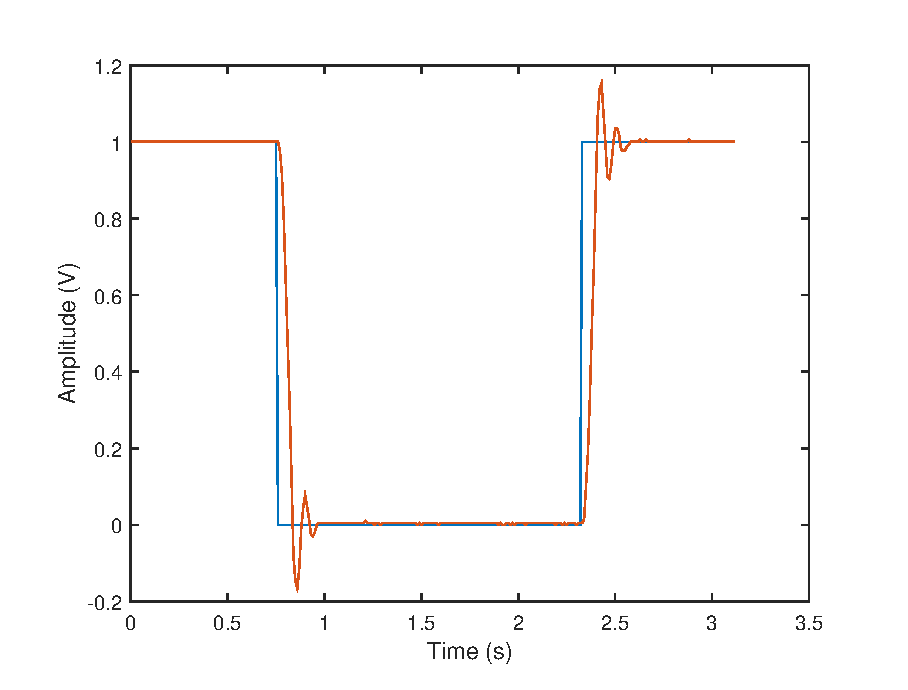
\includegraphics[scale=0.5]{fig21}
		\caption{Time domain response of controlled system with $K_v = 2$ and $K_P = 62$}
	\end{minipage}
	\hspace{1cm}
	\begin{minipage}{7cm}
		\centering
		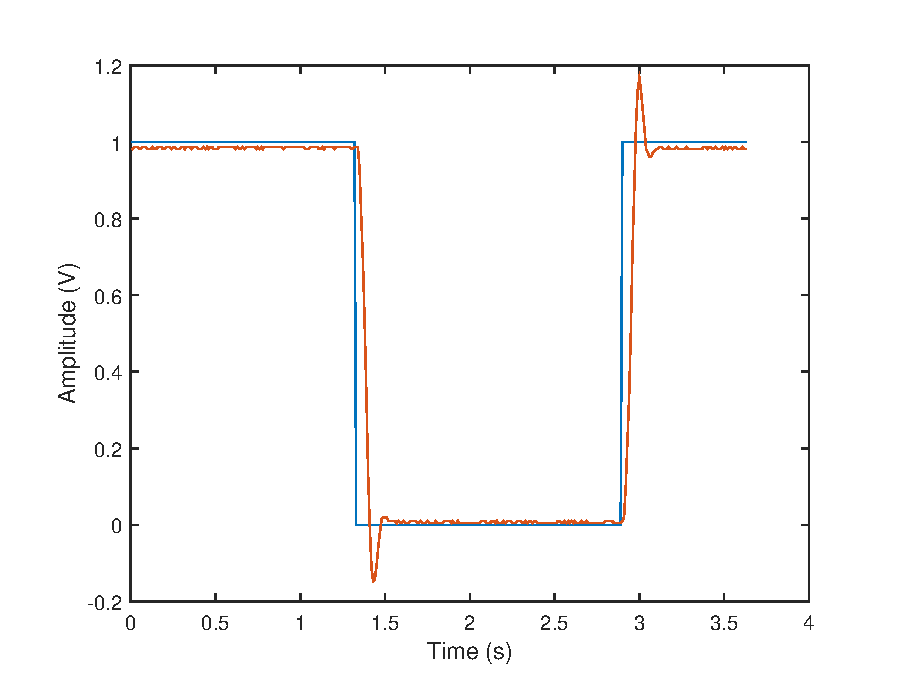
\includegraphics[scale=0.5]{fig22}
		\caption{Time domain response of controlled system with $K_v = 1$ and $K_P = 30$}
	\end{minipage}
\end{figure}

\begin{figure}[H]
	\hspace{0.5cm}
	\begin{minipage}{7cm}
		\centering
		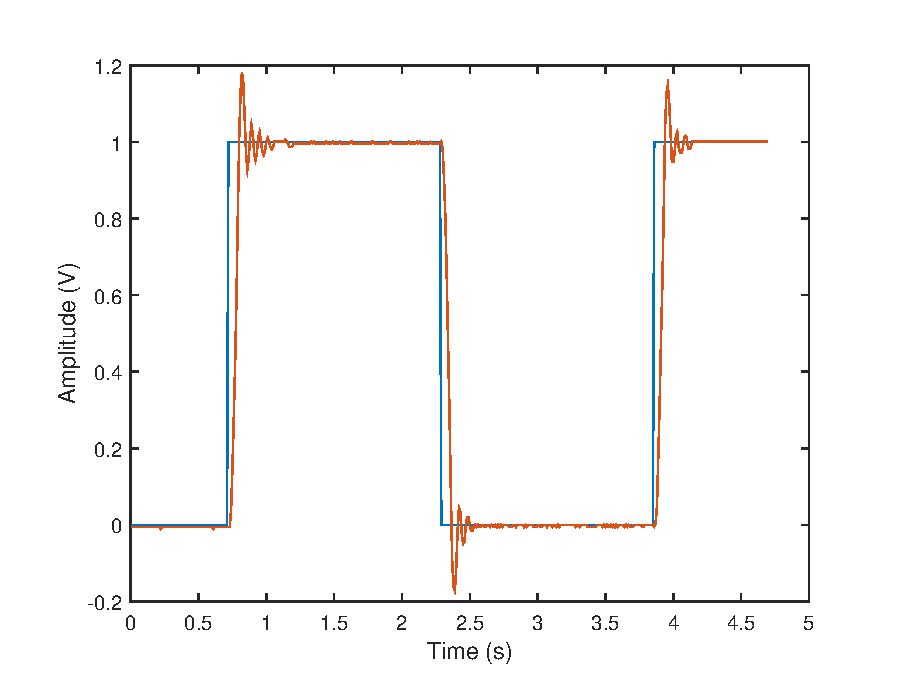
\includegraphics[scale=0.5]{fig23}
		\caption{Time domain response of controlled system with $K_v = 3$ and $K_P = 90$}
	\end{minipage}
	\hspace{1cm}
	\begin{minipage}{7cm}
		\centering
		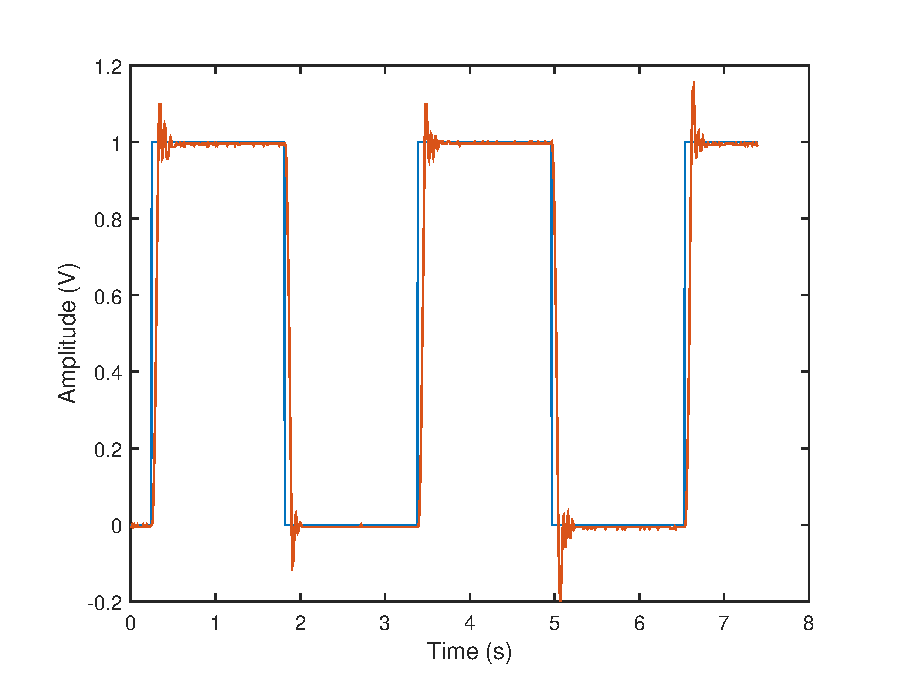
\includegraphics[scale=0.5]{fig24}
		\caption{Time domain response of controlled system with $K_v = 4$ and $K_P = 100$}
	\end{minipage}
\end{figure}

\begin{table}[H]
	\centering
	\caption{Performance metrics for controller with velocity and postion feedback control.}
	\begin{tabular}{crrrr}
		\toprule
		\textbf{Performance} 	& $K_v = 1$ & $K_v=2$ 	& $K_v=3$ 	& $K_v=4$ \\
		\textbf{Metric} 		& $K_P=30$ 	& $K_P=62$ 	& $K_P=90$	& $K_P=100$ \\
		\midrule
		$t_d$ & 0.06 & 0.055 & 0.06 & 0.06\\
		$t_r$ & 0.09 & 0.10 & 0.09 & 0.09\\
		$M_P$ & 16 & 16 & 16 & 16\\
		$t_s$ & 0.25 & 0.28 & 0.39 & 0.305\\
		\bottomrule
	\end{tabular}
\end{table}

\newpage

Generating a constant signal in open loop mode, data was collected from the tacho and position sensors for 1$\si{\volt}$ intervals from -3$\si{\volt}$ to 3$\si{\volt}$, which was used to determine the transfer function $G_{tacho}$. The plots of the collected data can be seen in Figure 18. The position and tachometer signals in the frequency range, $Y(s)_{tacho}$ and $Y(s)_{pos}$ respectively, are linked as follows:
\begin{align*}
	Y(s)_{tacho} = G(s)_{tacho} \cdot Y(s)_{pos}
\end{align*}

We note that the tachometer simply measures the angular velocity of the motor, and the position sensor measures the position of the motor. Hence, in the time domain, we see that the link between the two sensors can be described as:
\begin{align*}
y(t)_{tacho} = K_T \cdot \frac{d}{dt} \cdot y(t)_{pos}
\end{align*}

\begin{figure}[H]\hspace{-10mm}
	\centering
	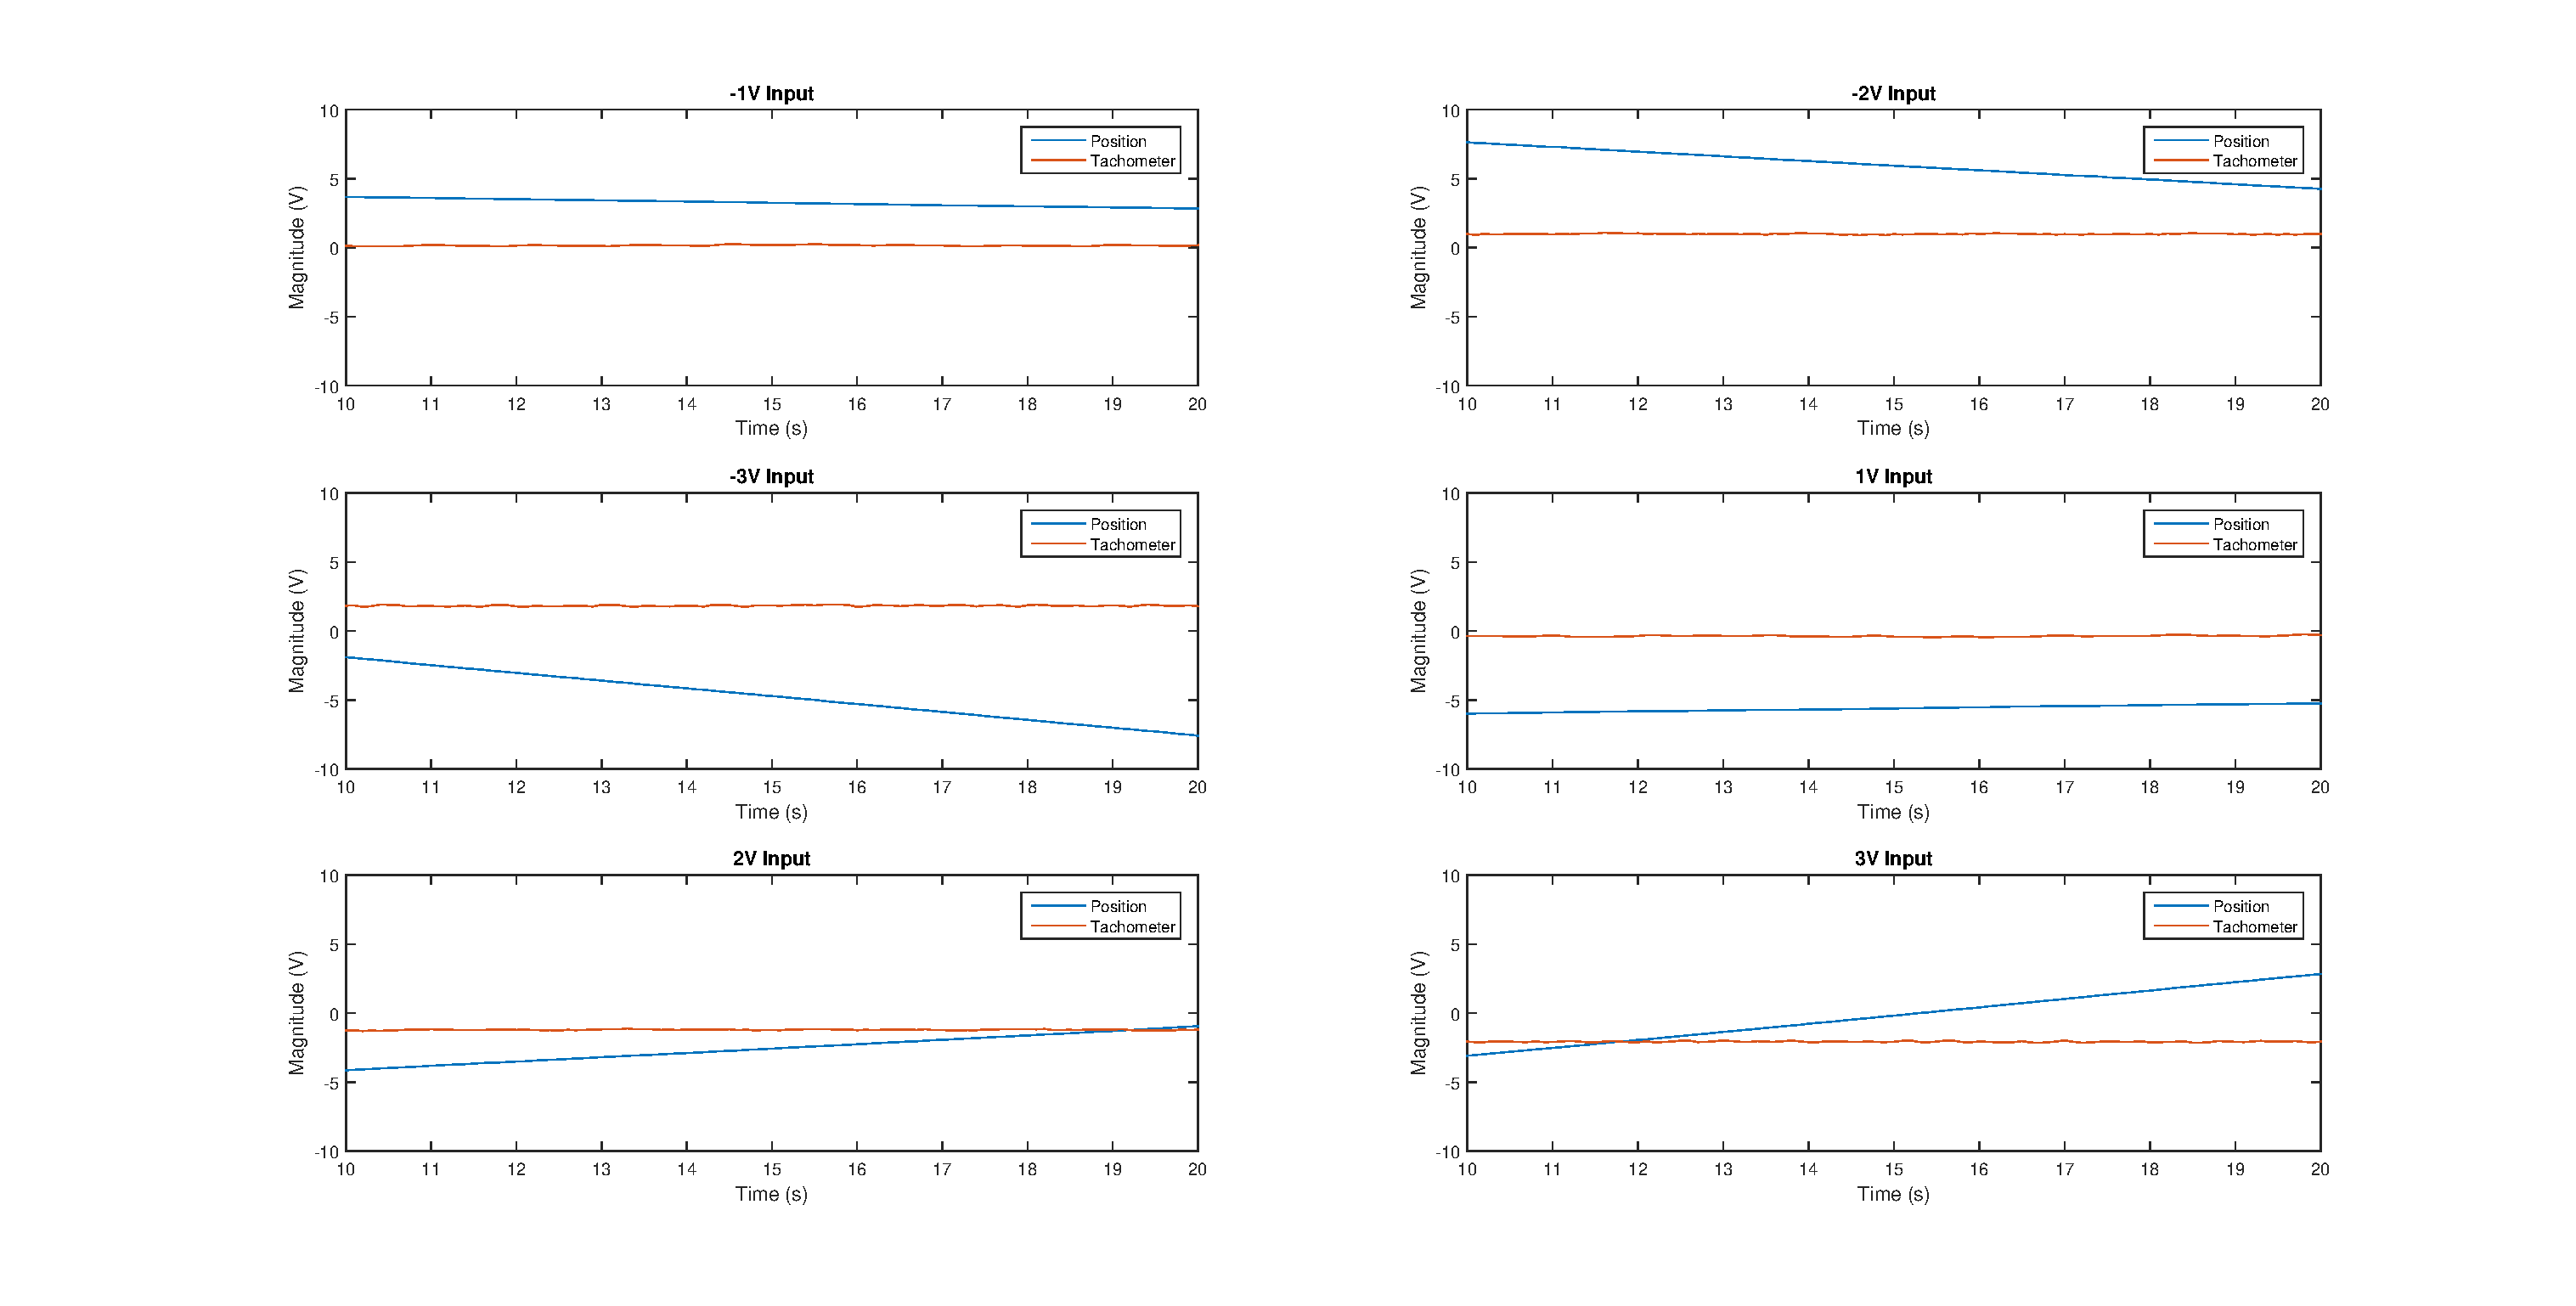
\includegraphics[scale=0.25]{fig20}
	\caption{Plot of captured data for position and tachometer.}
\end{figure}

The parameter $K_T$ is a scaling factor, since the position sensor is separated by some gearing ratio. Taking the Laplace transform, we get that:
\begin{align*}
	\mathscr{L} \{ y(t)_{tacho} \} = \mathscr{L} \{ K_T \cdot \frac{d}{dt} \cdot y(t)_{pos} \}
\end{align*}

The transform gives us:
\begin{align*}
	\frac{Y(s)_{tacho}}{Y(s)_{pos}} = K_T \cdot s
\end{align*}

To find an estimate for the parameter $K_T$, the slope of each position curve seen in Figure 14 was estimated using linear regression. Further, the average value of the tachometer signal was calculated. The results for both can be seen in Table 5. The results of Table 5 were plotted in Figure 19 and linear regression was employed to determine an estimate for $K_T$. It was found that:
\begin{align*}
	K_T = 0.33
\end{align*}


\begin{figure}[H]
	\hspace{0.55cm}
	\begin{minipage}{7cm}
		\captionof{table}{Slope of position curve and average tachometer value.}
		\begin{tabular}{ccc}
			\toprule
			\textbf{Input}  & \textbf{Slope} & \textbf{Average}\\
			\textbf{Voltage} ($\si{\volt}$) & \textbf{of Position} & \textbf{Tacho}\\
			\midrule
			\ 1	&	\ 0.7521  & 	-0.3500\\
			\ 2	&	\ 3.2020	&   -1.2090\\
			\ 3	&	\ 5.6900	&   -2.0580\\
			-1	&	-0.8058	&    \ 0.1461\\
			-2	&	-3.3729	&    \ 0.9900\\
			-3	&	-5.9900 &   \ 1.8400\\
			\bottomrule
		\end{tabular}
	\end{minipage}
	\hspace{1cm}
	\begin{minipage}{7cm}
		\centering
		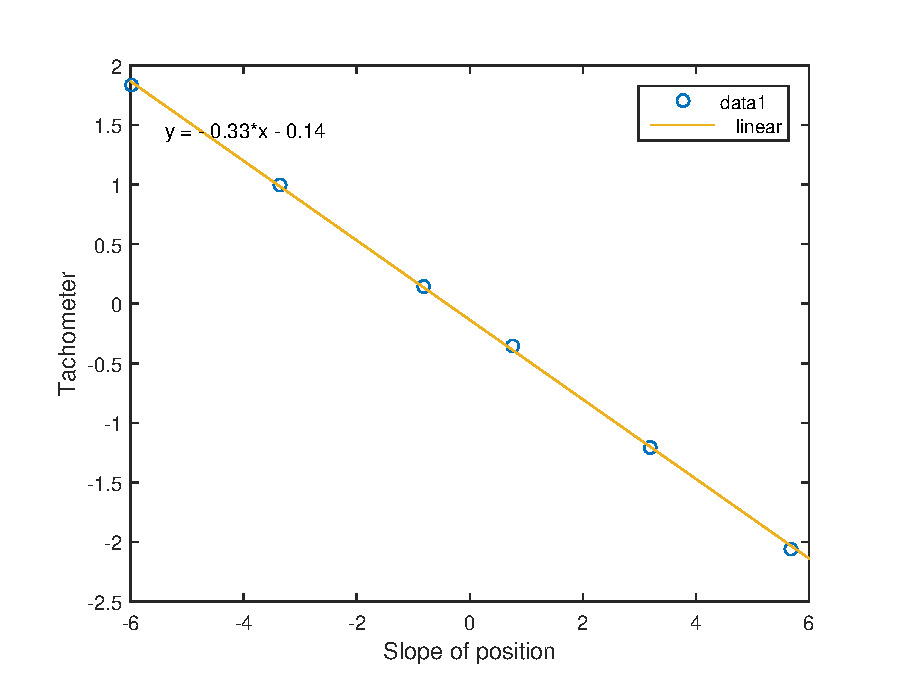
\includegraphics[scale=0.5]{fig19}
		\caption{Linear regression applied to a plot of the data in Table 4 to determine $K_T$.}
	\end{minipage}
\end{figure}

The open loop transfer function shown in equation (1) was used to determine an open loop transfer function for the system with velocity feedback $K_v = 2$:
\begin{align}
	G_O(s) = \frac{1.91}{s(0.029s^2 + 2.26)}
\end{align}

Equation (8) was then used to determine a theoretical closed loop transfer function with both proportional position feedback $K_P$, and $K_v = 2$:
\begin{align}
	H(s) = \frac{K_P \cdot 65.86}{s^2 + 77.93s + K_P \cdot 65.86}
\end{align}

Similarly to section 2, we find that $\zeta = 0.5038$ for a 16\% overshoot. Now, using equation (9) we can find the value of $\omega_n$ as:
\begin{align*}
	\omega_n = \frac{77.93}{2 \cdot 0.5038} = 77.34
\end{align*}

Solving the polynomial $s^2 + 2(0.5038)(77.34)s + (77.34)^2 = 0$, we get the following two poles:
\begin{align}
	p_1 = -38.96 - i66.80\\
	p_2 = -38.96 + i66.80
\end{align}

The magnitude condition $|K_P||G_O(s)| = 1$ is used to find the gain $K_P$ required to place the poles found in (11) and (12). The open loop transfer function $G_O(s)$ is from equation (8). Rearranging the magnitude condition and substituting a pole, we get:
\begin{align*}
	|K_P| = \frac{|0.029s^2 + 2.26s|}{1.91} = \frac{|-173.43 + i0.02137|}{1.91} = 90.80
\end{align*}

The root locus plot of the open loop function shown in equation (8) can be seen in Figure 20. Compared to the root locus plot found in section 2, the plots are very similar. The principal differences are that the poles are further apart, and the breakaway point is further from the origin. Both plots show inherently stable systems. Using root locus plot in Figure 20, it was found that the gain, $K_P$, to place the poles shown in (10) and (11) was found to be 90.80. This matched exactly with the theoretically calculated gain using the magnitude condition, however, was approximately 50\% larger than the experimentally determined value of $K_P = 62$ shown in Table 4. This overestimation is consistent with that of section 2 - which may be due to calculative errors.

\begin{figure}[H]
	\centering
	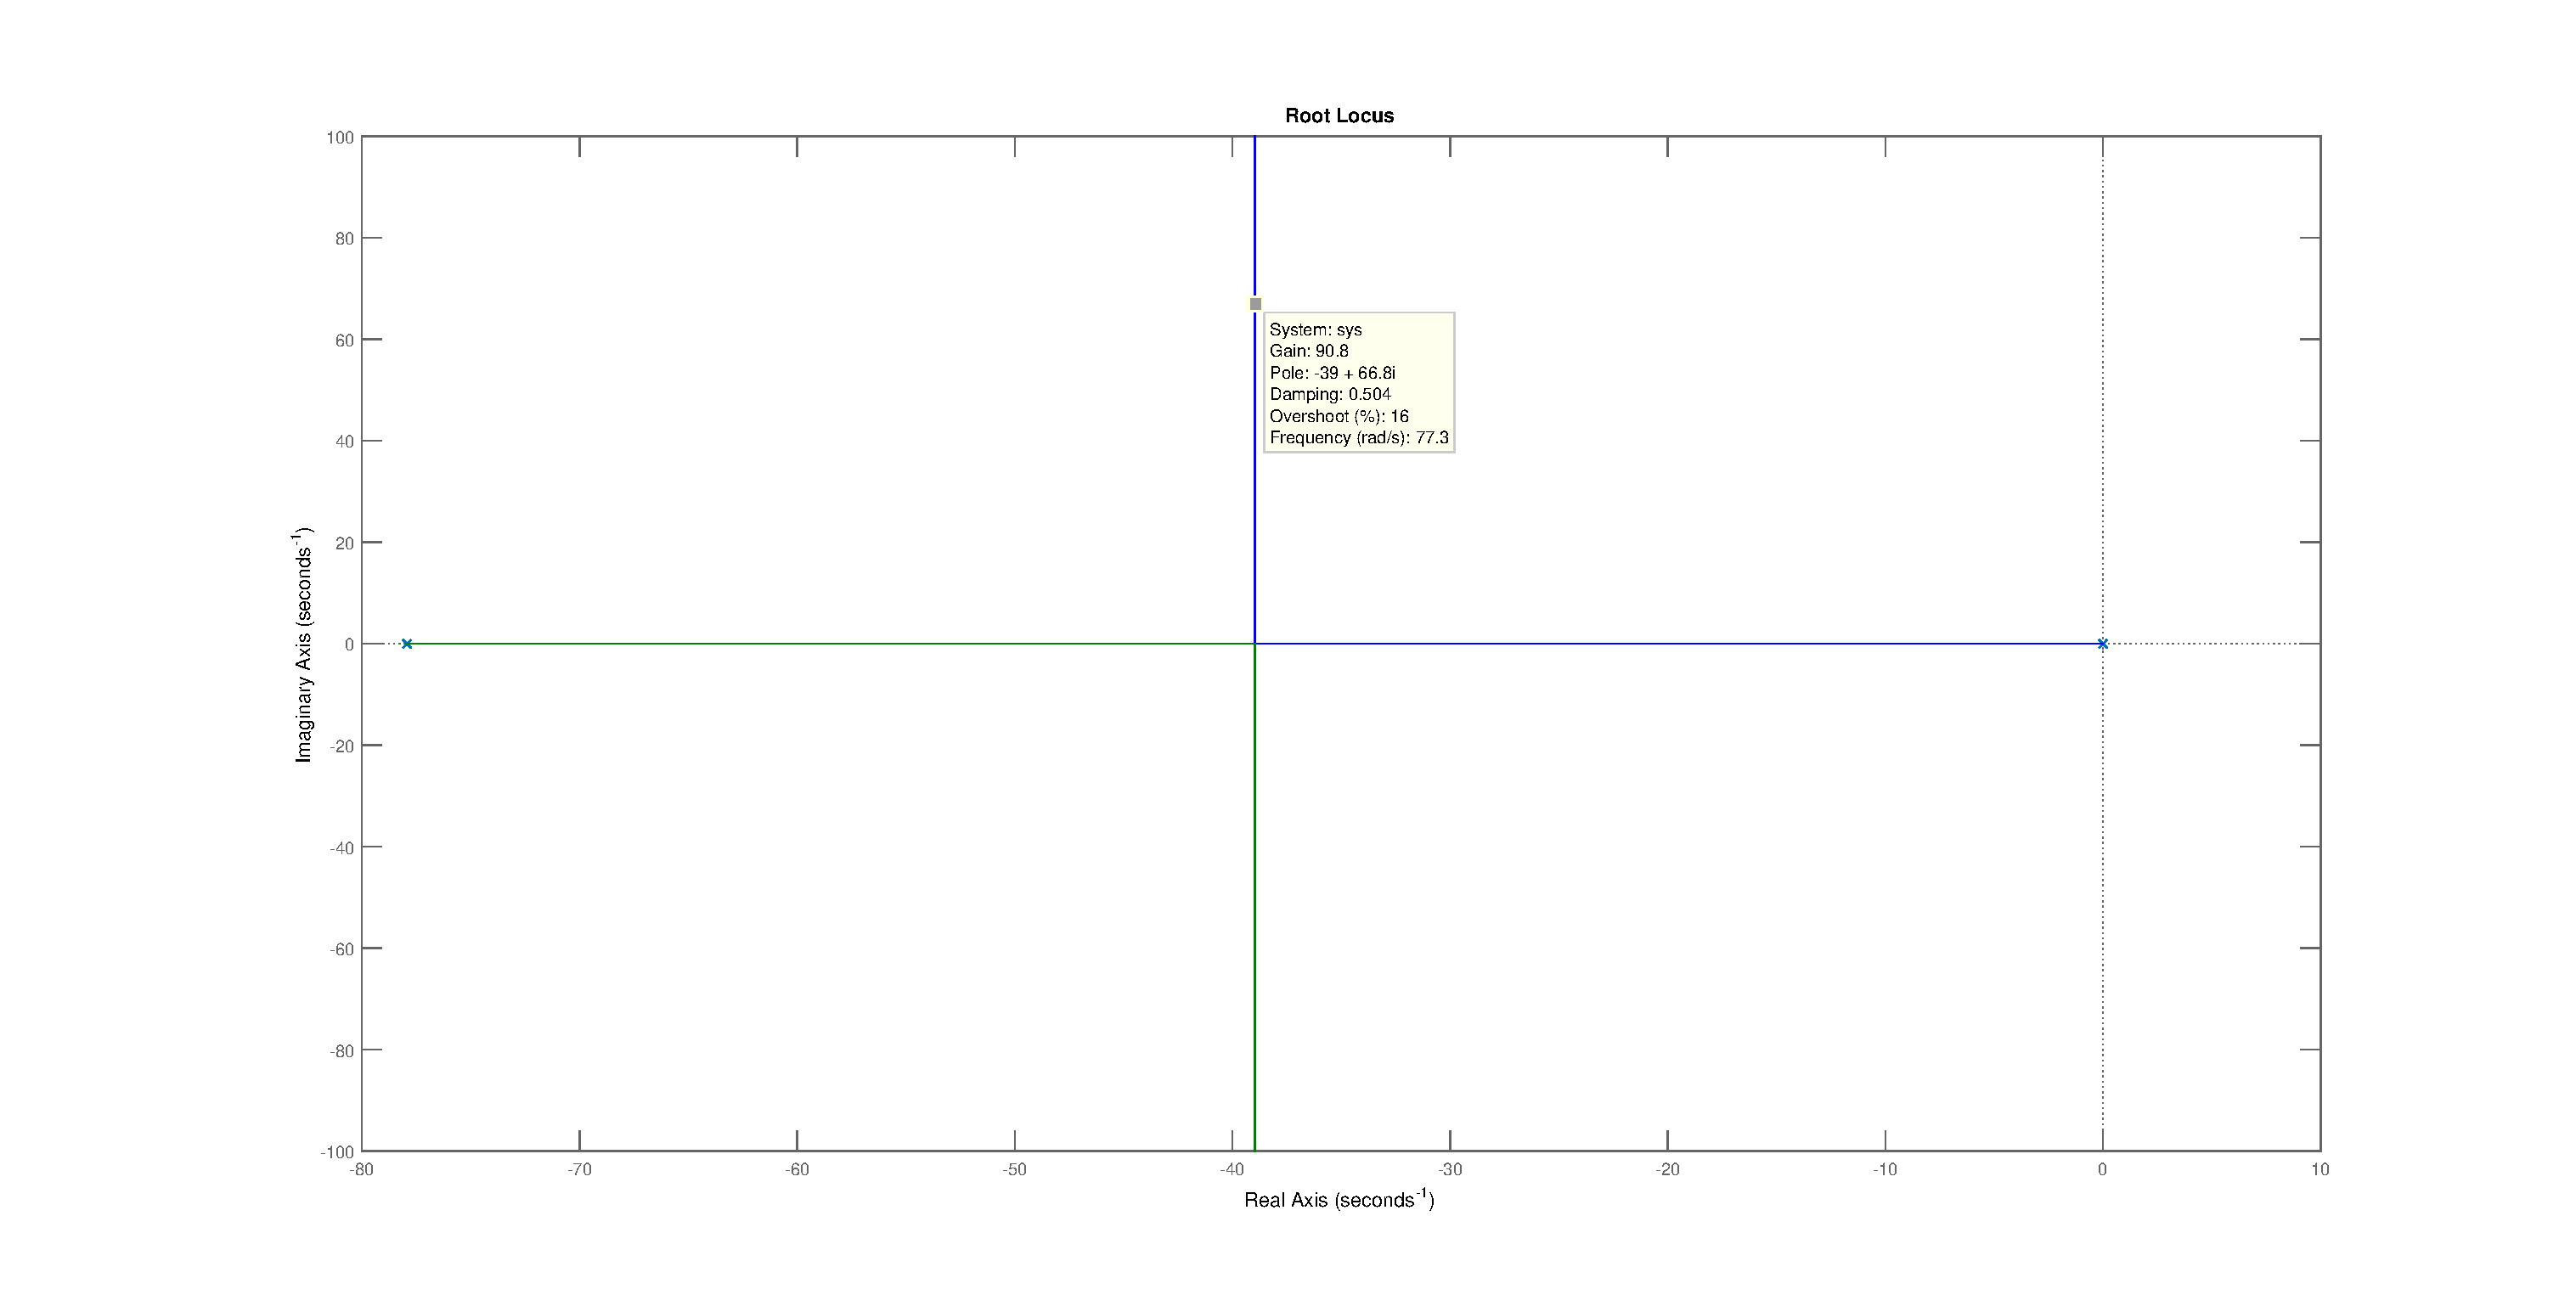
\includegraphics[scale=0.25]{fig25}
	\caption{Root locus diagram of open loop system with velocity feedback control.}
\end{figure}
%----------------------------------------------------------------------------------------
%	SECTION 4
%----------------------------------------------------------------------------------------

\section{Lead Compensator Design}

%----------------------------------------------------------------------------------------
%	SUBSECTION 1
%----------------------------------------------------------------------------------------

\subsection{Objective}

Theoretically design a Lead Compensator to control the electric servo motor, and analyse the performance 
%----------------------------------------------------------------------------------------
%	SUBSECTION 2
%----------------------------------------------------------------------------------------

\subsection{Procedure and Results}

The model used for this section is the open loop model shown in equation (1), which is:
\begin{align*}
	G_P(s) = \frac{1.91}{s(0.029s + 1)}
\end{align*}

Assuming that $K_c\alpha = K = 20$, we need to find the static velocity constant, $K_v$. Ogata tells us that:
\begin{align*}
	\lim_{s \rightarrow 0} s \cdot G_C(s) \cdot G_P(s) = K_v
\end{align*}

Where $G_C(s)$ is the Lead Compensator and is given by:
\begin{align*}
	G_C(s) = K_C \cdot \alpha \cdot \frac{Ts + 1}{\alpha Ts + 1}
\end{align*}

Hence, we get that:
\begin{align*}
	K_v &= \lim_{s \rightarrow 0} s \cdot \frac{63.43}{s(s + 33.67)} \cdot \frac{Ts+1}{\alpha Ts + 1}\\
		&= \frac{63.43 \cdot 20 \cdot 1}{33.67}\\
		&= 37.67
\end{align*}

\begin{figure}[H]
	\hspace{0.5cm}
	\begin{minipage}{7cm}
		\centering
		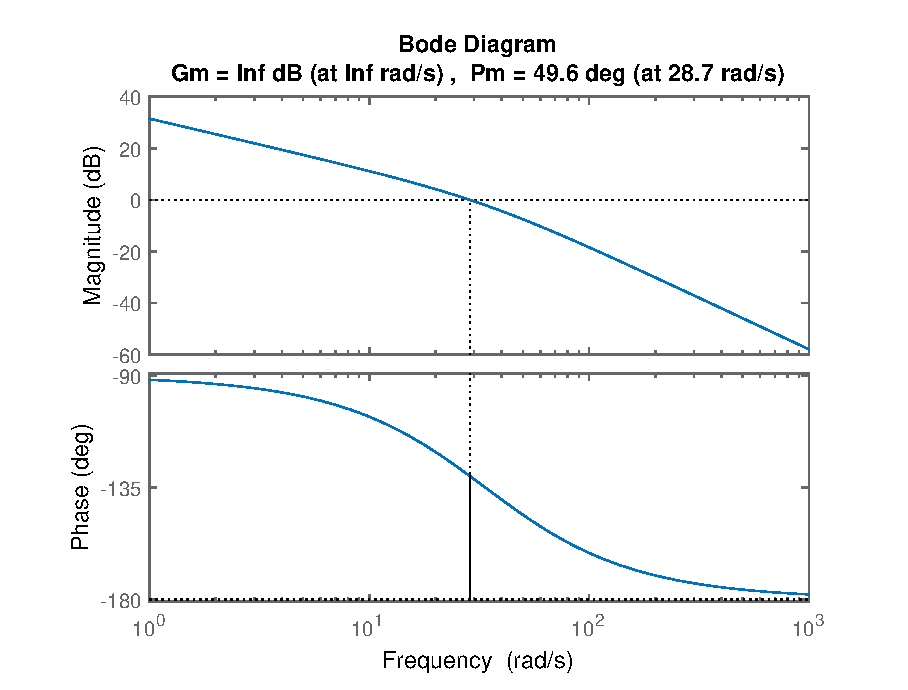
\includegraphics[scale=0.5]{fig11}
		\caption{Bode plot showing the Phase margin as 49.6$\si{\degree}$ for the uncontrolled system.}
	\end{minipage}
	\hspace{1cm}
	\begin{minipage}{7cm}
		\centering
		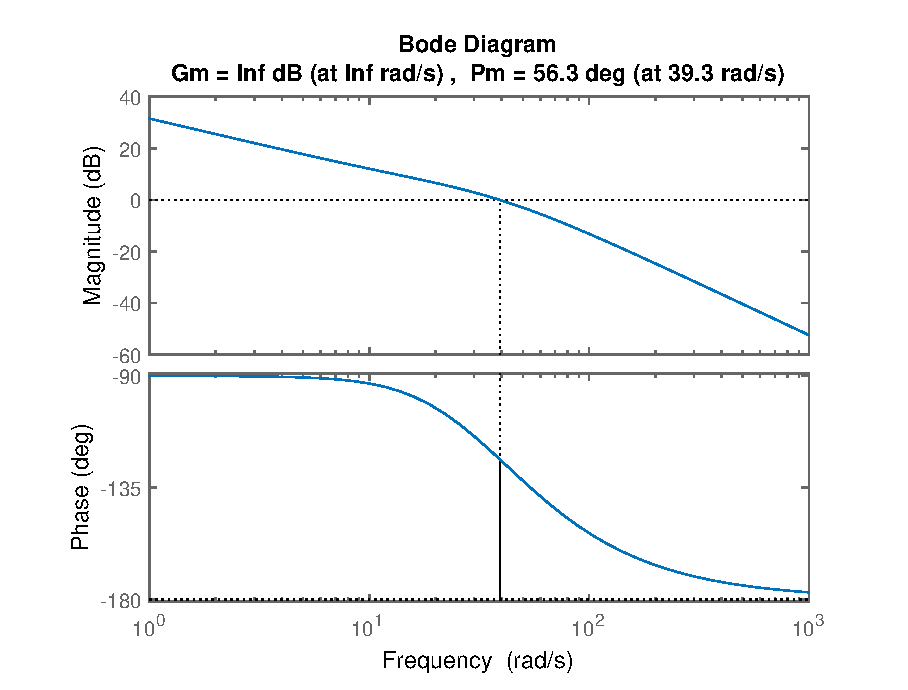
\includegraphics[scale=0.5]{fig12}
		\caption{Bode plot showing the Phase margin as 55.8$\si{\degree}$ for the system with Lead Compensation applied.}
	\end{minipage}
\end{figure}

Analysing the margin plot of the system $K \cdot G_P$ we see that the phase margin, $P_m$, is 49.6$\si{\degree}$. This is shown in Figure 21. The phase to be added to the system is $60\si{\degree} - 49.6\si{\degree} = 10.4\si{\degree}$. An additional 7.5$\si{\degree}$ margin means 17.9$\si{\degree}$ of additional phase margin is required. Solving for $\alpha$, we find that:
\begin{align*}
	\alpha = \frac{1 - \sin(17.9 \si{\degree})}{1 + \sin(17.9 \si{\degree})} = 0.5298
\end{align*}

From this it is found that $\omega_n = 22.84\si{\radian\per\second}$, which can be used to determine $T$ as follows:
\begin{align*}
	T = \frac{1}{\omega_n \cdot \sqrt{\alpha}} = 0.06015
\end{align*}

Given these parameters, the lead compensator controller is given by:
\begin{align}
	G_C(s) = 37.75 \cdot \frac{s + 16.6251}{s + 31.3799}
\end{align}

The phase margin of the system $G(s) = G_C(s) \cdot G_P(s)$ is approximately 55.8$\si{\degree}$, shown in Figure 22. The total controlled system $G(s)$, had the following parameters for the lead compensator implementation seen in LabView:
\begin{align*}
	a &= 31.38\\
	b &= 37.75\\
	c &= -556.81
\end{align*}

The compensator was entered into LabView and the step response of the system can be seen in Figure 23. The delay time, $t_d$, rise time, $t_r$, overshoot, $M_P$, and the settling time were estimated from the plot and are reported in Table 6.

\begin{table}[H]
	\centering
	\caption{Performance metrics of Lead Compensator controller.}
	\begin{tabular}{cr}
		\toprule
		\textbf{Parameter} & \textbf{Estimation}\\
		\midrule
		$t_d$ ($\si{\second}$) & 0.05 \\
		$t_r$ ($\si{\second}$) & 0.1 \\
		$M_P$ (\%) & 0 \\
		$t_s$ ($\si{\second}$) & 0.2 \\
		\bottomrule
	\end{tabular}
\end{table}

\begin{figure}[H]
	\hspace{0.5cm}
	\begin{minipage}{7cm}
		\centering
		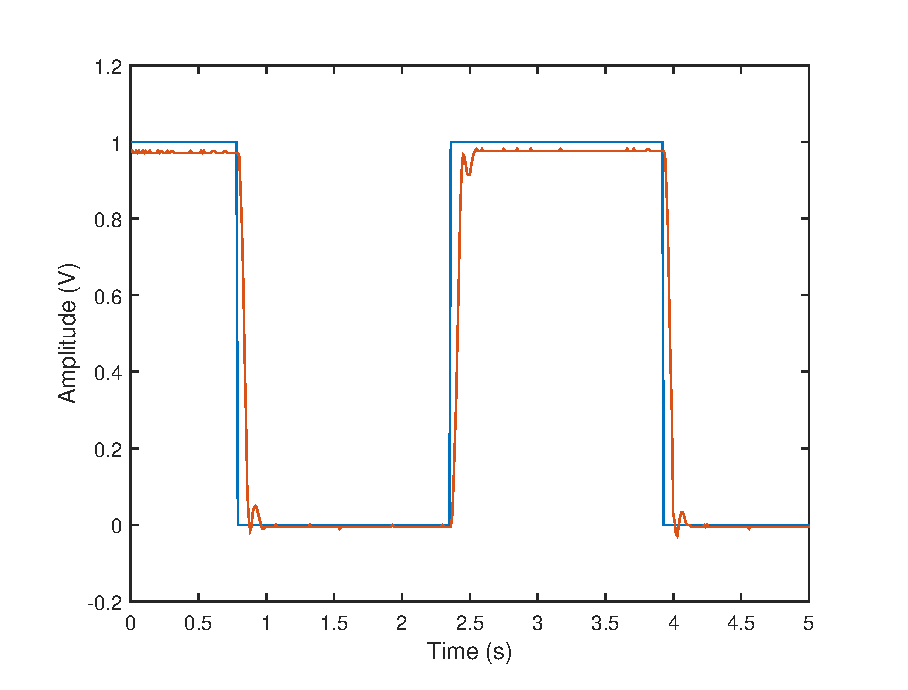
\includegraphics[scale=0.5]{fig13}
		\caption{Step response of system with Lead Compensator controller determined in equation (8).}
	\end{minipage}
	\hspace{1cm}
	\begin{minipage}{7cm}
		\centering
		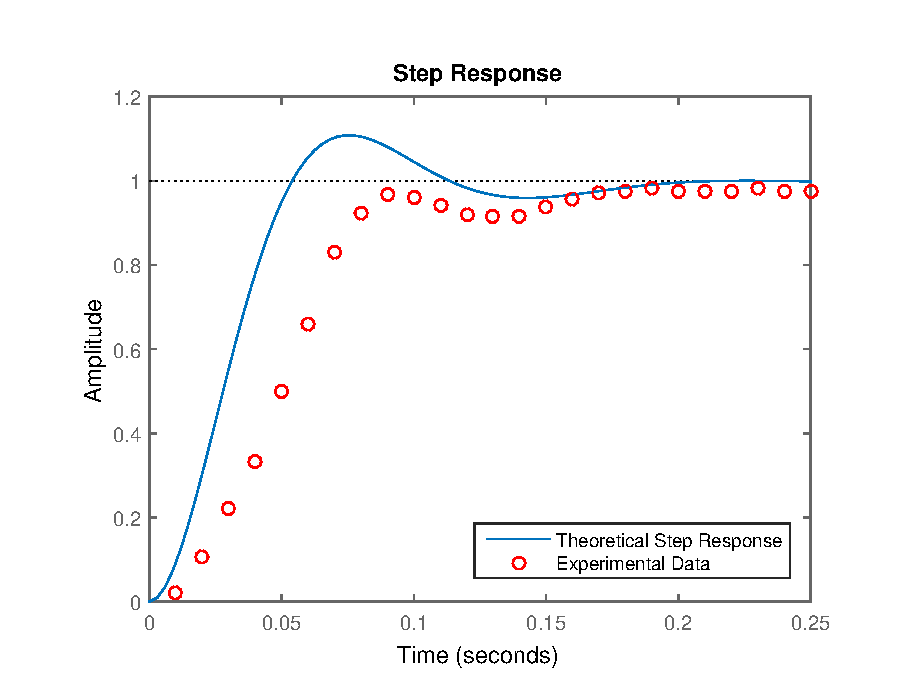
\includegraphics[scale=0.5]{fig14}
		\caption{Simulated step response of the Lead Compensator design shown in equation (8), plotted alongside captured experimental data of actual response.}
	\end{minipage}
\end{figure}

The transfer function for the lead compensator controller imposed on the system with feedback, was determined to be:
\begin{align*}
	H(s) = \frac{2185.79s + 37967.17}{s^3 + 63.6s^2 + 3193.53s + 37967.17}
\end{align*}

This was used to run a simulated step response in MATLAB, which was compared to experimental data. Figure 24 shows the results. The simulated data and the actual data are very close for this lead compensator design. To date this method of control has provided the most accurate results and the best performance in terms of delay, rise, overshoot, and settling times.
%----------------------------------------------------------------------------------------
%	SECTION 5
%----------------------------------------------------------------------------------------

\section{PID Control}

%----------------------------------------------------------------------------------------
%	SUBSECTION 1
%----------------------------------------------------------------------------------------

\subsection{Objective}

Implement P, PI and PID controllers for the system, tuning controller parameters using Ziegler Nichols tuning algorithm.

%----------------------------------------------------------------------------------------
%	SUBSECTION 2
%----------------------------------------------------------------------------------------

\subsection{Procedure and Results}

An step input signal between 0$\si{\volt}$ and 0.1$\si{\volt}$ was input to the system. The proportional gain was increased until the system became critically stable. The gain at which the system was critically stable was:
\begin{align*}
	K_{cr} = 55
\end{align*}

The time domain response of the system can be seen in Figure 17. The critical period $P_{cr}$ was found to be:
\begin{align*}
	P_{cr} = 0.1
\end{align*}

\begin{figure}[H]
	\centering
	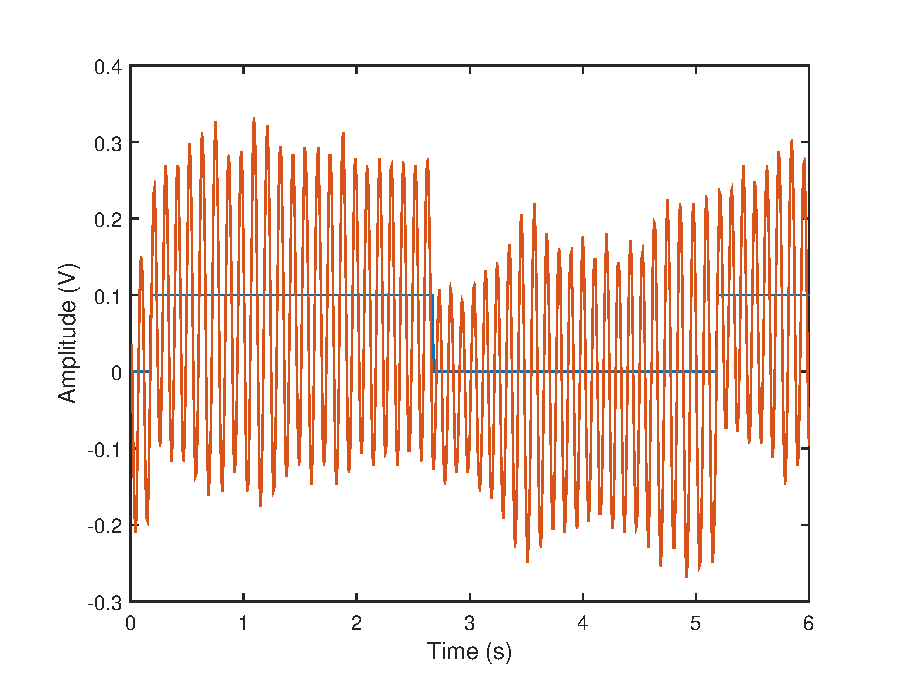
\includegraphics[scale=0.5]{fig15}
	\caption{Electromechanical system critically unstable at $K_{cr} = 55$.}
\end{figure}

Table 5 shows the parameters for the P, PI, and PID controller were calculated using the estimated values for $K_{cr}$ and $P_{cr}$. The closed loop transfer function for the P controller is:
\begin{align}
	H(s) = \frac{52.52}{0.029s^2 + s +52.52}
\end{align}

 \begin{table}[H]
	\centering
	\caption{Tuned controller parameters for P, PI, and PID controllers.}
	\begin{tabular}{lccc}
		\toprule
		\textbf{Controller} & $P = K_P$ & $I = \frac{K_P}{10 \cdot T_i}$ & $D = K_P \cdot T_d$\\
		\midrule
		\textbf{P} & 27.50 & 0.00 & 0.00\\
		\textbf{PI} & 24.75 & 29.71 & 0.00\\
		\textbf{PID} & 33.00 & 66.00 & 0.41\\
		\bottomrule
	\end{tabular}
\end{table}

The closed loop transfer function for the PI controller is:
\begin{align}
H(s) = \frac{47.27s 567.27}{0.029s^3 +s^ 47.27s 567.27}
\end{align}

The closed loop transfer function for the PID controller is:
\begin{align}
H(s) = \frac{0.7878s^2 + 63.02s + 1600}{0.029s^3 + 1.7878s^2 + 63.02s + 1600}
\end{align}

Each of the controllers, P, PI, and PID, were implemented in LabView, and data collected on the step response of each. Further, each of the 3 transfer functions (13), (14), and (15) were simulated in MATLAB capturing their step responses. Figures 26, 27, and 28 show the simulated step responses and the experimental data of the implemented controllers. Performance metrics were estimated from each of the experimental data plots, the results of which can be seen in Tables 10, 11, and 12. 

\begin{figure}[H]
	\hspace{0.5cm}
	\begin{minipage}{7cm}
		\centering
		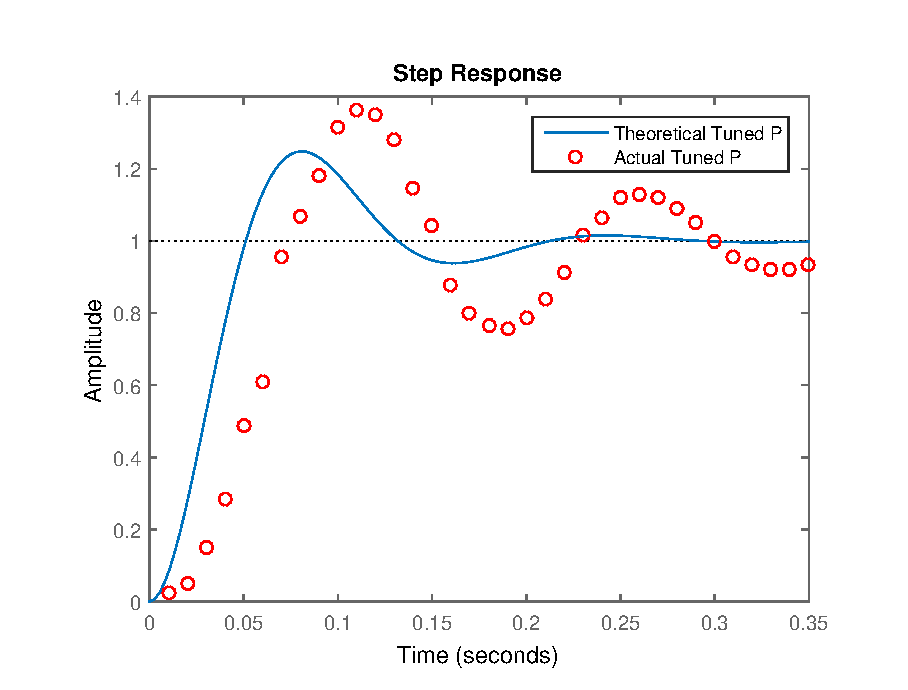
\includegraphics[scale=0.5]{fig16}
		\caption{Simulated step response of system with theoretically determined P controller, compared with actual controlled system response.}
	\end{minipage}
	\hspace{1cm}
	\begin{minipage}{7cm}
		\captionof{table}{Performance metrics of tuned P controller.}
		\begin{tabular}{cr}
			\toprule
			\textbf{Parameter} & \textbf{Estimation}\\
			\midrule
			$t_d$ & 0.06 \\
			$t_r$ & 0.085 \\
			$M_P$ & 14 \\
			$t_s$ & 0.42 \\
			\bottomrule
		\end{tabular}
	\end{minipage}
\end{figure}

\begin{figure}[H]
	\hspace{0.5cm}
	\begin{minipage}{7cm}
		\centering
		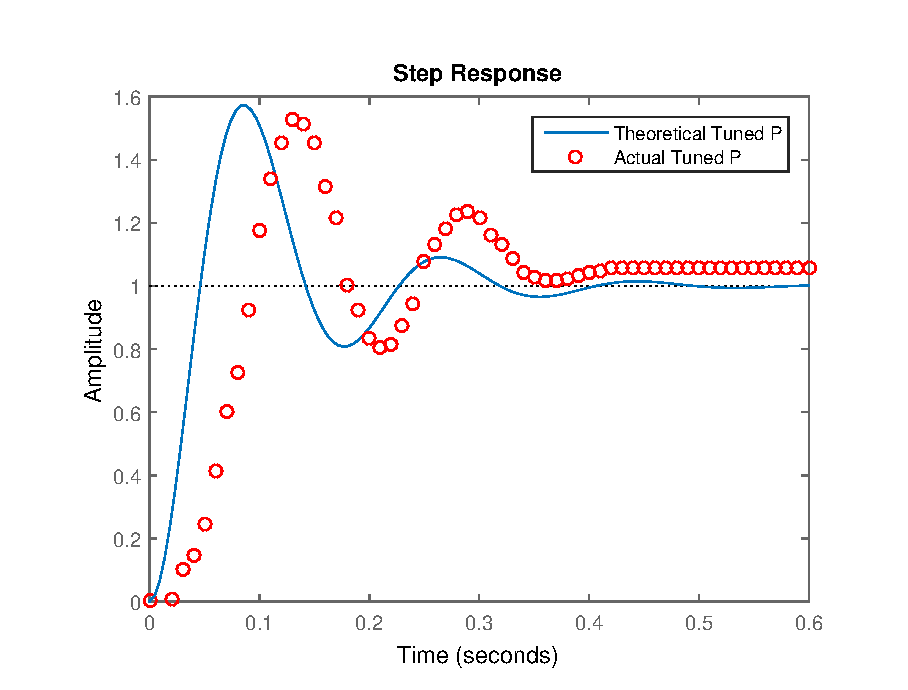
\includegraphics[scale=0.5]{fig17}
		\caption{Simulated step response of system with theoretically determined PI controller, compared with actual controlled system response.}
	\end{minipage}
	\hspace{1cm}
	\begin{minipage}{7cm}
		\captionof{table}{Performance metrics of tuned PI controller.}
		\begin{tabular}{cr}
			\toprule
			\textbf{Parameter} & \textbf{Estimation}\\
			\midrule
			$t_d$ & 0.08\\
			$t_r$ & 0.105\\
			$M_P$ & 15\\
			$t_s$ & 0.48\\
			\bottomrule
		\end{tabular}
	\end{minipage}
\end{figure}

Each of the theoretically simulated responses are more optimistic than the actual system performance, however, provide a fairly accurate representation of the real system. It must be noted that the PID control is of the worst form of control in terms of the observed performance metrics shown in Tables 8, 9, and 10. This may simply be an artefact of improper calculation and implementation or perhaps is more indicative of the fact that PID may not be a suitable control type for this problem.

\begin{figure}[H]
	\hspace{0.5cm}
	\begin{minipage}{7cm}
		\centering
		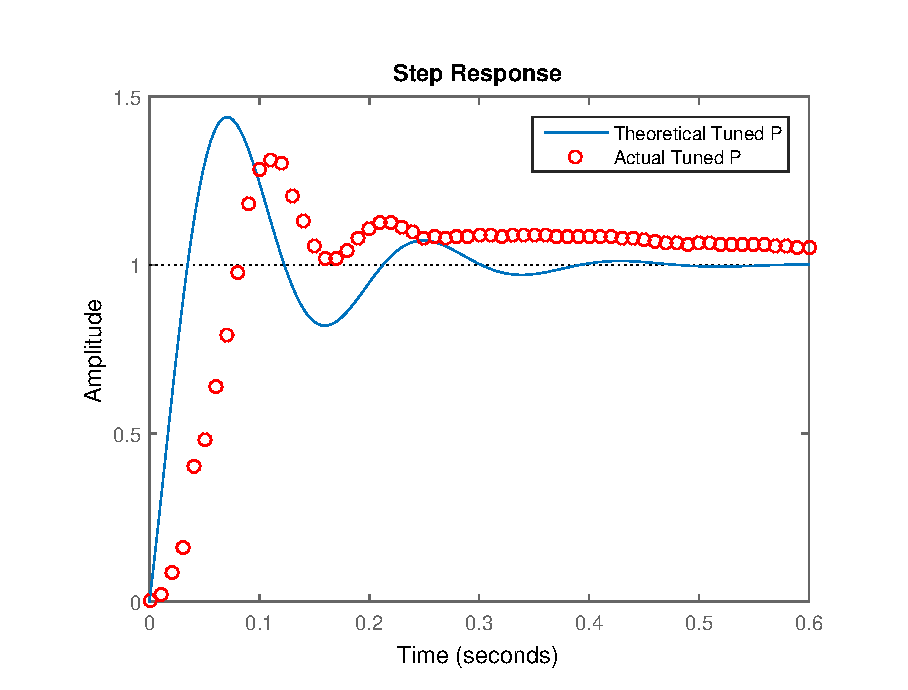
\includegraphics[scale=0.5]{fig18}
		\caption{Simulated step response of system with theoretically determined PID controller, compared with actual controlled system response.}
	\end{minipage}
	\hspace{1cm}
	\begin{minipage}{7cm}
		\captionof{table}{Performance metrics of tuned PID controller.}
		\begin{tabular}{cr}
			\toprule
			\textbf{Parameter} & \textbf{Estimation}\\
			\midrule
			$t_d$ & 0.07\\
			$t_r$ & 0.09\\
			$M_P$ & 30\\
			$t_s$ & 1.00\\
			\bottomrule
		\end{tabular}
	\end{minipage}
\end{figure}

%----------------------------------------------------------------------------------------
%	SECTION 4
%----------------------------------------------------------------------------------------

\section{Conclusions}

Generally, the series of practicals was deeply informative and provided a comprehensive overview of the techniques employed when implementing a variety of control methods. In particular the frequency response determination of the open loop transfer functions is an invaluable skill set, however, could have been made stronger by providing the user some tolerances on the parameters they needed to find. Further, the design and implementation of the Lead Compensator provided solid insight to the design process and subsequent implementation. As an external student, I found the work load for this series of practicals difficult to manage. Admittedly there were other projects that I were undertaking at the same time I was undertaking this, however, I remained in the lab until 7 - 8pm on the last two nights in order to get the results completed. Finally, the write up for this practical was a monumental effort, however, this is a fourth year subject and I assume that this is what is expected? 

\newpage

\section{References}
Ogata, K. (2010). \textit{Modern Control Engineering}. Pearson Education Inc.

\end{document}